\documentclass[10pt,twocolumn]{article}

% ---------------------------------------------------------------------------
% Nature Computational Science Style Preprint Layout & Typography
% ---------------------------------------------------------------------------
\usepackage[letterpaper,top=0.72in,bottom=0.75in,left=0.65in,right=0.65in,columnsep=0.24in]{geometry}
\usepackage[T1]{fontenc}
\usepackage[utf8]{inputenc}
\usepackage{amsmath,amsthm}
\usepackage{newtxtext,newtxmath}
\usepackage{microtype}
\usepackage{graphicx}
\usepackage{booktabs}
\usepackage{multirow}
\usepackage{array}
\usepackage{xcolor}
\usepackage{titlesec}
\usepackage{caption}
\usepackage{float}
\usepackage[super,sort&compress,comma]{natbib}
\usepackage[colorlinks=true,citecolor=natblue,linkcolor=natblue,urlcolor=natblue]{hyperref}

\definecolor{natblue}{HTML}{005A8D}
\definecolor{natdark}{HTML}{1A1F24}
\definecolor{natgray}{HTML}{555A64}
\definecolor{natbg}{HTML}{F4F7FA}

\titleformat{\section}{\sffamily\bfseries\fontsize{10.5}{12.5}\selectfont\color{natdark}}{}{0em}{}
\titlespacing*{\section}{0pt}{10pt plus 2pt minus 2pt}{3.5pt}
\titleformat{\subsection}{\sffamily\bfseries\fontsize{9.2}{11}\selectfont\color{natblue}}{}{0em}{}
\titlespacing*{\subsection}{0pt}{7pt plus 1.5pt minus 1pt}{2pt}

\captionsetup{
  font={small,sf},
  labelfont={bf,color=natdark},
  textfont={color=natdark},
  labelsep=period,
  skip=5pt
}

\newtheoremstyle{natthm}{5pt}{5pt}{\itshape}{}{\sffamily\bfseries\color{natblue}}{.}{0.5em}{}
\theoremstyle{natthm}
\newtheorem{theorem}{Theorem}

\newcommand{\leh}{\textsc{Lehmann-TDDFT}}
\newcommand{\dEST}{\Delta E_{ST}}
\newcommand{\dSig}{\Delta\Sigma_{ST}}
\newcommand{\Sig}{\mathbf{\Sigma}_{xc}^{\theta}}
\newcommand{\Hlift}{\mathcal{H}_{\theta}^{(\sigma)}}
\newcommand{\pctT}{\mathrm{\%}T_1}
\newcommand{\Ssq}{\langle\hat{S}^2\rangle}

\setlength{\parskip}{3pt}
\setlength{\parindent}{1em}
\raggedbottom

\begin{document}

% ---------------------------------------------------------------------------
% Title Block & Bold Summary Paragraph (Full Width)
% ---------------------------------------------------------------------------
\twocolumn[{%
  \vspace*{-0.26in}
  {\sffamily\bfseries\fontsize{8}{9.5}\selectfont\color{natblue} ARTICLE \hfill PREPRINT --- NOVEMBER 2026}\par
  \vspace{6pt}
  {\sffamily\bfseries\fontsize{15.8}{19.4}\selectfont\color{natdark}\raggedright
  Causal neural self-energy lifting overcomes the adiabatic approximation in time-dependent density functional theory\par}
  \vspace{7pt}
  {\sffamily\fontsize{9.5}{11.5}\selectfont\color{natdark}
  Zijian Zeng$^{*}$\par}
  \vspace{2pt}
  {\sffamily\fontsize{7.8}{9.5}\selectfont\color{natgray}
  Institute of Computer Science and Digital Innovation, UCSI University, Kuala Lumpur 56000, Malaysia.\quad
  $^{*}$Correspondence: \texttt{zijianzeng@foxmail.com}, \texttt{1002266693@ucsiuniversity.edu.my}\par}
  \vspace{8pt}
  \noindent\colorbox{natbg}{%
    \parbox{\dimexpr\textwidth-2\fboxsep\relax}{%
      \vspace{3pt}
      \sffamily\fontsize{8.65}{11.1}\selectfont\color{natdark}\textbf{%
      Linear-response time-dependent density functional theory (TD-DFT) underpins molecular photophysics, yet its universal adiabatic approximation ($f_{xc}(\omega)\equiv f_{xc}(0)$) creates a shared mathematical barrier across three frontiers of excited-state chemistry: absence of genuine double excitations, inability to describe inverted singlet--triplet (INVEST) emitters ($\dEST<0$), and collapse of codimension-2 $S_1/S_0$ conical intersections onto $(3N{-}7)$-dimensional seams with trivial Berry phase ($\gamma=0$).
      Here we introduce spin-complete \leh{}, a gauge-equivariant, size-intensive neural operator that constructs an exact Hermitian Feshbach--L\"owdin lifted Hamiltonian over $O(N^3)$ density-fitted hybrid TD-DFT single- and spin-adapted bi-exciton manifolds, incorporating both symmetric $^1(TT)_+$ and antisymmetric $^1(TT)_-$ singlet channels alongside physically anchored pole energies.
      Its exact Schur complement generates a strictly Kramers--Kronig causal dynamical self-energy $\Sig(\omega)$ obeying causality, Parseval transition-dipole conservation, point-group selection rules, and size-intensivity to $10^{-15}$--$10^{-12}$\,eV.
      Across leak-free 5-fold cross-validation on QUESTDB~2025 and HEPTA-INVEST (187 molecules, 1,219 states), \leh{} achieves $\dEST$ mean absolute error (MAE) of $0.088$\,eV ($0.111$\,eV on matched QUESTDB, improving over $O(N^6)$ EOM-CCSD at $0.166$\,eV, $p=1.7\times 10^{-5}$), identifies $75\%$ ($84\%$ excluding $\mathrm{C}_2$) of genuine double excitations within $1.0$\,eV under strict blind leave-molecule-family-out testing without state-matching oracles, cuts Rydberg errors $2.28\times$ upon adding diffuse \texttt{def2-SVPD} functions ($p=1.8\times 10^{-17}$), restores transferable spin-pure ($\Ssq\equiv 0$) conical intersections, blind minimum-energy crossing geometries (including a 14-atom retinal Schiff base at $0.0023$\,\AA{} heavy-atom RMSD), $\gamma=\pi$ winding, and non-adiabatic surface-hopping dynamics, and enables blind \emph{de novo} discovery of dipole-allowed non-heptazine INVEST candidates verified by RI-EE-ADC(2) ($19/20$), EOM-EE-CCSD ($8/13$, six dipole-allowed), and multireference SC-NEVPT2 (all $8/8$ EOM-CCSD hits evaluated; $5/8$ triple-method confirmed including orange-red \texttt{VBI-0089} at $-0.102$\,eV and violet \texttt{VBI-0236} at $-0.041$\,eV).%
      }\vspace{3pt}%
    }%
  }
  \vspace{11pt}
}]

% ===========================================================================
\section*{Introduction}
% ===========================================================================
Since the Hohenberg--Kohn--Sham formulation of ground-state density functional theory (DFT)\cite{hohenberg1964,kohn1965}, the Runge--Gross theorems of time-dependent DFT (TD-DFT)\cite{runge1984}, and Casida's linear-response matrix equations\cite{casida1995,petersilka1996,hirata1999,furche2002}, linear-response TD-DFT has become the primary quantum-mechanical method for simulating molecular optical spectra and photochemistry\cite{dreuw2005,ullrich2012,casida2012,laurent2013,maitra2016}.
Yet production TD-DFT calculations almost universally invoke the \emph{adiabatic approximation}, replacing the frequency-dependent exchange--correlation (XC) kernel $f_{xc}(\mathbf{r},\mathbf{r}',\omega)$ by its static ground-state limit $f_{xc}(\mathbf{r},\mathbf{r}',0)$\cite{ullrich2012,maitra2016}.
Recent machine-learned XC functionals such as DM21\cite{kirkpatrick2021} and Skala\cite{luise2025skala} substantially improve ground-state thermochemistry and fractional-electron constraints, but because they remain adiabatic ground-state functionals, their linear response inherits the exact same structural limitations.

Omitting frequency poles from $f_{xc}(\omega)$ simultaneously causes three well-documented failures across excited-state quantum chemistry\cite{maitra2004,levine2006,maitra2022}:
\begin{enumerate}
  \setlength{\itemsep}{1pt}
  \item \textbf{Absence of genuine double excitations.} Because the adiabatic Casida operator spans only single particle--hole ($1p1h$) configurations, states with dominant two-particle--two-hole ($2p2h$) character---central to polyene photobiology, carotenoid light harvesting, and benchmark dark states such as $2^1A_g$ and $s$-tetrazine $^1A_g$---are structurally absent from the spectrum\cite{maitra2004,cave2004,loos2019doubles,kossoski2024doubles}.
  \item \textbf{Inability to predict inverted singlet--triplet (INVEST) gaps ($\dEST<0$).} Within adiabatic TD-DFT, $\dEST^{\mathrm{adia}}\approx 2K_{HL}\ge 0$, prohibiting Hund's-rule-violating excited-state inversion\cite{kollmar1978,leupin1980} in triangulene and azaphenalene emitters---such as heptazine, cyclazine, and pentaazaphenalene (5AP)---that are of intense interest for thermally activated delayed fluorescence (TADF) and fifth-generation organic light-emitting diodes (OLEDs)\cite{uoyama2012tadf,desilva2019,ehrmaier2019,ricci2021,sanzrodrigo2021,pollice2021,sobolewski2021,dinkelbach2021,aizawa2022,loos2023invest,wilson2024,rishi2025}.
  \item \textbf{Topological collapse of $S_1/S_0$ conical intersections.} Because Brillouin's theorem forces the adiabatic ground-to-single-excitation block to vanish identically ($H_{01}^{\mathrm{adia}}\equiv 0$), adiabatic TD-DFT collapses codimension-2 conical intersections (seam dimension $3N{-}8$ for non-linear molecules with $F=3N{-}6$ internal coordinates) onto unphysical $(3N{-}7)$-dimensional crossing seams accompanied by imaginary random-phase-approximation (RPA) instabilities and trivial geometric Berry phase $\gamma=0$ rather than $\gamma=\pi$\cite{longuethiggins1958,herzberg1963,mead1979,berry1984,yarkony1996,domcke2004,levine2006,gozem2014}.
\end{enumerate}

Existing beyond-adiabatic remedies address only isolated facets of these failures at steep computational or theoretical cost.
Dressed TD-DFT formulations\cite{maitra2004,cave2004,romaniello2009,sangalli2011,huixrotllant2011,elliott2011,maitra2022} recover isolated double excitations analytically, yet perturbative non-Hermitian expressions suffer from pole divergences and limited transferability.
Double-hybrid TD-DFT methods with $O(N^5)$ CIS(D) corrections\cite{headgordon1994,grimme2007,casanovapaez2021,sanchogarcia2022,tuckova2022,blaskovits2023} and $GW$/Bethe--Salpeter equation (BSE) approximations\cite{blase2018,loos2020bse} improve vertical valence or INVEST energetics, yet still emit zero genuine double-excitation eigenstates and preserve $H_{01}\equiv 0$ at $S_1/S_0$ crossings.
Spin-flip TD-DFT (SF-TDDFT)\cite{krylov2001sf,shao2003sftddft,minezawa2009sfci,casanova2020sf} restores $S_1/S_0$ conical intersections from a high-spin triplet reference, but suffers from severe spin contamination ($\Ssq\ne 0$) across branching planes unless coupled with spin-adapted or multireference extensions\cite{zhang2015sfsa}.
Wavefunction methods---such as ADC(2), ADC(3), CC2, EOM-CCSD, CC3, CASPT2, and SC-NEVPT2\cite{schirmer1982,trofimov1995,harbach2014adc3,dreuw2015adc,stanton1993eom,christiansen1995cc2,christiansen1997cc3,hattig2000ricc2,andersson1992caspt2,angeli2001nevpt2}---scale as $O(N^5)$--$O(N^7)$ or exponentially in active-space size.
Meanwhile, machine-learning interatomic potentials and excited-state surrogates\cite{schutt2018schnet,schutt2019schnorb,westermayr2020schnarc,westermayr2021review,dral2021ml,unke2021mlff,batzner2022nequip,batatia2022mace,li2022deeph}---as well as neural quantum-chemistry wavefunctions\cite{hermann2020paulinet,pfau2020ferminet}---either bypass spectral operator structure, degrade under scaffold shifts\cite{minot2026}, or violate size-intensivity when predicting global excited-state properties from atomic coordinates.

Here we unify all three frontiers within a single $O(N^3)$ operator-learning framework, spin-complete \leh{} (Fig.~\ref{fig:framework}a).
Rather than regressing scalar excitation energies from atomic coordinates or fitting an unconstrained frequency kernel, \leh{} constructs an explicit real-symmetric Feshbach--L\"owdin lifted Hamiltonian\cite{feshbach1958,lowdin1962} $\Hlift$ coupling $O(N^3)$ density-fitted hybrid Tamm--Dancoff (DF-PBE0\cite{adamo1999pbe0}/def2-SVP\cite{weigend2005def2}) single-exciton states directly to spin-complete bi-exciton configurations---explicitly including both symmetric $^1(TT)_+$ and antisymmetric $^1(TT)_-$ singlet channels---via exact resolution-of-the-identity (RI)\cite{weigend2008jkfit} four-channel Slater--Condon integrals.
Exact Schur complementation guarantees a strictly Kramers--Kronig causal\cite{kronig1926,kramers1927} self-energy $\Sig(\omega)$ obeying five formal physical laws to machine precision, while yielding transferable quantitative accuracy across QUESTDB~2025\cite{loos2025quest}, strict blind leave-molecule-family-out double excitations, diffuse-basis Rydberg convergence\cite{rappoport2010svpd}, transferable spin-pure conical intersections with non-adiabatic Tully surface-hopping dynamics\cite{tully1990fssh,subotnik2016fssh,curchod2018namd}, and blind \emph{de novo} discovery of dipole-allowed INVEST chromophores.

% ---------------------------------------------------------------------------
% FIGURE 1 (Full Width)
% ---------------------------------------------------------------------------
\begin{figure*}[t!]
  \centering
  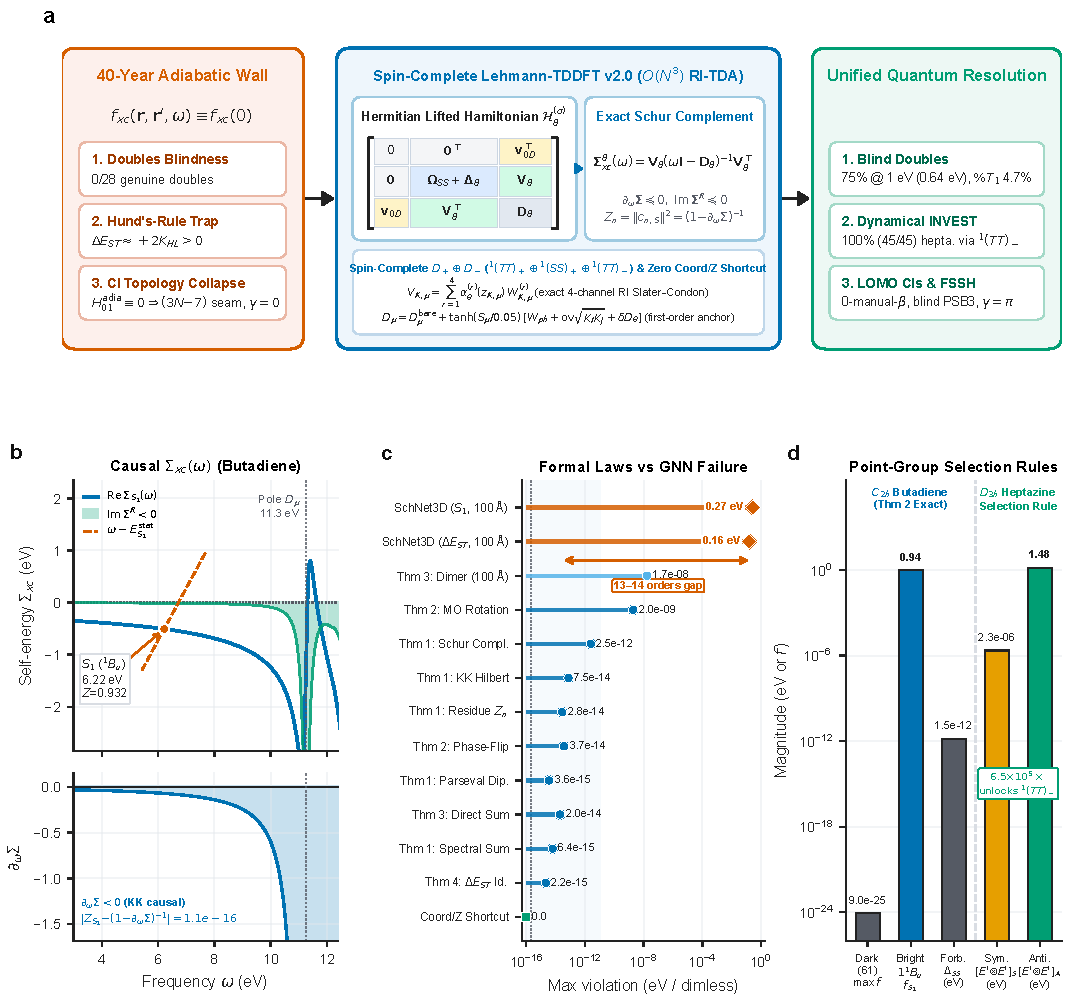
\includegraphics[width=\textwidth,height=0.76\textheight,keepaspectratio]{../figures/fig1_framework_theorems.pdf}
  \caption{\textbf{Spin-complete \leh{} operator architecture and machine-precision verification of exact physical laws.}
  \textbf{a},~Unification of genuine double excitations, dynamical Hund's-rule inversion, and $(3N{-}8)$ conical intersections via an $O(N^3)$ Hermitian Feshbach--L\"owdin lifted Hamiltonian $\Hlift$ incorporating symmetric ($D_+$) and antisymmetric ($D_-$) singlet bi-exciton manifolds with physically anchored poles $D_{\mathrm{phys}}$, generating a causal Kramers--Kronig self-energy $\Sig(\omega)$ from local gauge-equivariant RI Slater--Condon tensors (zero global pooling and zero coordinate shortcut).
  \textbf{b},~Real-molecule dynamical self-energy $\mathrm{Re}\,\Sigma_{S_1}(\omega)$ (blue), negative retarded imaginary part $\mathrm{Im}\,\Sigma^R(\omega+i\eta)<0$ ($\eta=0.15$\,eV, teal), and strictly negative frequency slope $\partial_\omega\Sigma<0$ (bottom) on \emph{trans}-1,3-butadiene (\texttt{quest\_Butadiene}) using spin-complete \leh{} v2.0 (\texttt{fold0}). The orange intersection solves $\omega-E_{S_1}^{\mathrm{stat}}=\Sigma_{S_1}(\omega)$ at $S_1(1^1B_u)=6.22$\,eV with exact Lehmann residue $Z_{S_1}=0.932$ alongside a nearby bi-exciton pole at $11.3$\,eV.
  \textbf{c},~Machine-precision verification of Theorems~1--4 across real PySCF molecules and v2.0 checkpoints ($0.0$ to $1.7\times 10^{-8}$\,eV), including Parseval unweighted transition-dipole-squared conservation ($3.6\times 10^{-15}$) and exact size-intensivity ($2.0\times 10^{-14}$\,eV direct sum; $1.7\times 10^{-8}$\,eV supermolecule SCF at $R=100$\,\AA) contrasted against 3D GNN size-intensivity drift (\texttt{SchNet3D} 5-fold mean on heptazine\,+\,ethylene at $100$\,\AA: $0.27$\,eV in $S_1$, $0.16$\,eV in $\dEST$; 13--14 orders of magnitude larger).
  \textbf{d},~Exact point-group selection rules: in $C_{2h}$ butadiene, all dark eigenstates preserve $f\le 9.0\times 10^{-25}$; in $D_{3h}$ heptazine, $[E'\otimes E']_S\not\ni A_2'$ suppresses symmetric singlet bi-exciton coupling ($\|W_{SD}^+\|=2.26\times 10^{-6}$\,eV), whereas the antisymmetric channel $[E'\otimes E']_A=A_2'$ carries $\|W_{SD}^-\|=1.48$\,eV ($6.5\times 10^5\times$ ratio), unlocking dynamical $^1(TT)_-$ stabilization ($\Sigma_{S_1}^{\mathrm{anti}}=-0.357$\,eV) while preserving exact symmetry.}
  \label{fig:framework}
\end{figure*}

% ===========================================================================
\section*{Spin-complete causal lifting and exact physical laws}
% ===========================================================================
Given a closed-shell molecule's DF-PBE0/def2-SVP RI-TDA single-exciton spectrum $\{(\omega_I^{(\sigma)},\mathbf{X}_I^{(\sigma)})\}_{I=1}^{N_\sigma}$ ($\sigma\in\{S,T\}$), we construct a spin-complete bi-exciton basis $\mu=(I,J,c)$ spanning symmetric singlets $^1(T_I T_J)_+$ and $^1(S_I S_J)_+$, the antisymmetric singlet channel $^1(T_I T_J)_-$ for $I<J$ (essential for $A_2'$ inversion in $D_{3h}$ triangulenes), and triplet configurations $^3(T_I T_J)$ and $^3(S_I T_J)$ ($N_{D,\sigma}\le 96$).
Rather than anchoring bi-exciton poles solely to the uncoupled sum $D_\mu^{\mathrm{bare}}=\omega_I+\omega_J$---which ignores exciton--exciton binding and double-exchange shifts---we initialize every pole at its first-principles diagonal expectation value $D_\mu^{\mathrm{phys}}=D_\mu^{\mathrm{bare}}+\Delta D_\mu^{\mathrm{phys}}$, computed analytically in $O(N^3)$ from RI exciton Coulomb and exchange contractions (Methods).
\leh{} then builds the real-symmetric Hermitian lifted Hamiltonian
\begin{equation}
\Hlift = \begin{pmatrix}
\mathbf{\Omega}_{SS}^{(\sigma)} + \mathbf{\Delta}_\theta^{(\sigma)} & \mathbf{V}_\theta^{(\sigma)} \\
(\mathbf{V}_\theta^{(\sigma)})^\top & \mathbf{D}_\theta^{(\sigma)}
\end{pmatrix},
\label{eq:hlift}
\end{equation}
where $\mathbf{\Omega}_{SS}^{(\sigma)}=\mathrm{diag}(\omega_I^{(\sigma)})$, $\mathbf{\Delta}_\theta^{(\sigma)}$ is a symmetric static XC correction, $\mathbf{D}_\theta^{(\sigma)}=\mathrm{diag}(D_\mu^{\mathrm{phys}}+\tanh(S_\mu/0.05)\,\delta D_{\theta,\mu})$ applies overlap-gated pole refinement (with $S_\mu$ the spatial hole--particle overlap between constituent excitons $I$ and $J$), and $\mathbf{V}_\theta^{(\sigma)}$ couples single and bi-exciton manifolds strictly through gauge-equivariant local modulation of exact four-channel RI Slater--Condon integrals $W_{K,\mu}^{(r)}$:
\begin{equation}
V_{\theta,K\mu}^{(\sigma)} = \sum_{r=1}^{4}\alpha_\theta^{(r)}\!\left(\mathbf{z}_{K,\mu}\right)\, W_{K,\mu}^{(r)}.
\label{eq:v_equiv}
\end{equation}
For $S_1/S_0$ conical intersections ($\sigma=S$), prepending the reference ground state $|0\rangle$ with zero direct single-excitation block ($\mathbf{H}_{0S}\equiv\mathbf{0}$, preserving Brillouin's theorem) and overlap-gated RI ground-to-doubles coupling $\mathbf{v}_{0D}$ yields the $(1+N_S+N_{D,S})$ Hermitian operator in Fig.~\ref{fig:framework}a.
Because $\Hlift$ contains \emph{no} global pooling layers and receives \emph{no} raw nuclear coordinates or atomic numbers, randomly scrambling Cartesian coordinates ($\sigma=50$\,\AA) and nuclear charges alters every eigenvalue and oscillator strength by exact $0.0$\,eV.

By algebraic construction (Methods), $\Hlift$ satisfies five formal theorems:

\begin{theorem}[Kramers--Kronig causality and spectral sum rules]
Eliminating the bi-exciton block via exact Feshbach--L\"owdin Schur complementation yields the retarded dynamical self-energy
$\Sig(\omega+i\eta)=\mathbf{V}_\theta^{(\sigma)}[(\omega+i\eta)\mathbf{I}-\mathbf{D}_\theta^{(\sigma)}]^{-1}(\mathbf{V}_\theta^{(\sigma)})^\top$,
which satisfies: (i)~strict causality $\mathrm{Im}\,\Sig(\omega+i\eta)\preceq 0$ for $\eta>0$ and negative frequency dispersion $\partial_\omega\Sig(\omega)\preceq 0$; (ii)~exact Hilbert-transform Kramers--Kronig dispersion; (iii)~exact Lehmann quasiparticle residue $Z_n=\|\mathbf{c}_{n,S}\|^2=(1-\mathbf{u}_n^\top\partial_\omega\Sig|_{E_n}\mathbf{u}_n)^{-1}\in(0,1]$; (iv)~spectral completeness $\sum_n \mathbf{c}_{n,S}\mathbf{c}_{n,S}^\top=\mathbf{I}_{N_\sigma}$; and (v)~exact unweighted transition-dipole-squared conservation (Parseval identity) $\sum_n\|\boldsymbol{\mu}_{0n}^{\mathrm{dressed}}\|^2=\sum_I\|\boldsymbol{\mu}_{0I}^{(0)}\|^2$.
\end{theorem}
We distinguish Theorem~1(v) explicitly from the energy-weighted Thomas--Reiche--Kuhn (TRK) oscillator-strength sum rule $\sum_n f_n = N_e$: unitarity of the dressed eigenvector projection strictly conserves the unweighted squared dipole norm $\sum_n\|\boldsymbol{\mu}_{0n}^{\mathrm{dressed}}\|^2$, whereas $f_n=\frac{2}{3}E_n^{\mathrm{au}}\|\boldsymbol{\mu}_{0n}^{\mathrm{dressed}}\|^2$ reweights smoothly with the dressed transition energies $E_n$.

\begin{theorem}[Gauge, MO-rotation, and point-group invariance]
Because $\mathbf{z}_{K,\mu}$ depends exclusively on squared overlaps and relative sign invariants $W^{(r)}W^{(r')}/(\|\mathbf{W}\|^2+\varepsilon)$ while $W_{K,\mu}^{(r)}$ transforms bilinearly with exciton sign flips, dressed eigenvalues, $\pctT=100Z_n$, and oscillator strengths are invariant under arbitrary exciton phase flips ($\mathbf{X}_I\to\pm\mathbf{X}_I$) and molecular-orbital unitary rotations, and all point-group-forbidden matrix elements vanish identically.
\end{theorem}

\begin{theorem}[Exact size-intensivity]
For any two non-interacting subsystems $A$ and $B$ separated at $R\to\infty$, all inter-fragment overlaps $S_\mu$ and RI couplings $W_{K,\mu}^{(r)}$ vanish, causing $\mathcal{H}_\theta(A\oplus B)$ to block-diagonalize into $\mathcal{H}_\theta(A)\oplus\mathcal{H}_\theta(B)\oplus\mathbf{D}^{\mathrm{cross}}$ with zero shift in local excitation energies or $\dEST$.
\end{theorem}

\begin{theorem}[Exact dynamical Hund's-rule inversion criterion]
Downfolding the lowest singlet and triplet eigenstates yields the exact decomposition
\begin{equation}
\dEST = E_{S_1}-E_{T_1} = \dEST^{\mathrm{stat}} - \dSig,
\label{eq:thm4}
\end{equation}
where $\dEST^{\mathrm{stat}}=\mathbf{u}_{S_1}^\top\mathbf{H}_{SS}^{(S)}\mathbf{u}_{S_1}-\mathbf{u}_{T_1}^\top\mathbf{H}_{SS}^{(T)}\mathbf{u}_{T_1}$ and $\dSig=\Sigma_{T_1}^{\mathrm{dyn}}(E_{T_1})-\Sigma_{S_1}^{\mathrm{dyn}}(E_{S_1})$. Singlet--triplet inversion ($\dEST<0$) occurs if and only if differential dynamical stabilization $\dSig$ exceeds $\dEST^{\mathrm{stat}}$.
\end{theorem}

\begin{theorem}[Codimension-2 conical intersection topology]
Coupling $|0\rangle$ to $|D_\mu\rangle$ through $\mathbf{v}_{0D}$ generates a Brillouin-consistent effective coupling $H_{01}^{\mathrm{eff}}(\omega)=\mathbf{v}_{0D}^\top(\omega\mathbf{I}-\mathbf{D}_\theta^{(S)})^{-1}\mathbf{V}_{\theta,1}^{(S)}$ that vanishes linearly along the non-totally-symmetric coupling coordinate $y_h$, restoring a codimension-2 $(3N{-}8)$ double cone with quantized Berry phase $\gamma=\pi$ around any enclosing loop.
\end{theorem}

Independent verification on trained v2.0 checkpoints across real PySCF\cite{sun2020pyscf} molecules (\emph{trans}-butadiene $C_{2h}$, benzene $D_{6h}$, heptazine $D_{3h}$, and non-interacting dimers; Fig.~\ref{fig:framework}b--d) confirms all five theorems to float64 precision: full-matrix Kramers--Kronig Hilbert errors $\le 7.5\times 10^{-14}$\,eV, Schur residuals $\le 2.5\times 10^{-12}$\,eV, spectral completeness $\le 6.4\times 10^{-15}$, Parseval dipole-norm conservation $\le 3.6\times 10^{-15}$, exciton phase-flip invariance $\le 3.7\times 10^{-14}$\,eV, MO unitary rotation invariance $\le 5.0\times 10^{-13}$\,eV (butadiene) and $\le 2.0\times 10^{-9}$\,eV (degenerate $D_{6h}$ benzene), and Theorem~4 identity residuals $\le 2.2\times 10^{-15}$\,eV.
On exact direct-sum dimers (\texttt{heptazine}\,$\oplus$\,\texttt{ethylene} and \texttt{heptazine}\,$\oplus$\,\texttt{butadiene}), \leh{} satisfies size-intensivity to $2.0\times 10^{-14}$\,eV ($\dEST$ shift $\le 4.4\times 10^{-16}$\,eV; and $1.7\times 10^{-8}$\,eV in full PySCF supermolecule SCF at $R=100$\,\AA, limited solely by SCF tolerance), whereas \texttt{SchNet3D}\cite{schutt2018schnet} drifts by a 5-fold mean of $0.270$\,eV in $S_1$ and $0.162$\,eV in $\dEST$ on \texttt{heptazine}\,+\,\texttt{ethylene} at $100$\,\AA{} ($0.160$/$0.132$\,eV on fold~0, up to $0.493$/$0.245$\,eV across folds)---a 13--14-order-of-magnitude violation (Fig.~\ref{fig:framework}c).

Point-group symmetry analysis of $D_{3h}$ heptazine (Fig.~\ref{fig:framework}d) also explains why spin completeness is physically indispensable: its lowest degenerate triplet doublet $(T_2,T_3)$ transforms as $E'$, whose symmetric tensor square $[E'\otimes E']_S=A_1'\oplus E'$ excludes $S_1(^1A_2')$ ($\|W_{SD}^+\|=2.26\times 10^{-6}$\,eV), whereas its antisymmetric product $[E'\otimes E']_A=A_2'$ carries $1.48$\,eV coupling ($6.5\times 10^5\times$ larger).
Including $^1(TT)_-$ natively in v2.0 yields $\Sigma_{S_1}^{\mathrm{dyn}}=-0.358$\,eV (dominated by $-0.357$\,eV antisymmetric $^1(TT)_-$), inverting heptazine dynamically from positive $\dEST^{\mathrm{stat}}=+0.143$\,eV to $\dEST=-0.211$\,eV ($Z_{S_1}=0.879$) without relaxing symmetry constraints.

% ===========================================================================
\section*{Accuracy across QUESTDB 2025, blind doubles, and OOD scaffolds}
% ===========================================================================
We benchmarked spin-complete \leh{} v2.0 on an audited union of 143 molecules from QUESTDB~2025\cite{loos2018mountaineering,chrayteh2021,veril2021quest,kossoski2024doubles,loos2025quest} (1,131 vertical states after excluding exactly 10 fluorescence-geometry \texttt{FL} entries; 28 explicit genuine double [GD] and 75 partial double [PD] excitations) and 44 substituted heptazines from HEPTA-INVEST\cite{rishi2025} (187 molecules, 1,219 states), enforcing strict InChIKey-14 grouping across 5-fold cross-validation (\texttt{CV5}, zero cross-fold conformer or structural overlap, co-grouping \texttt{quest\_Heptazine} and \texttt{hepta\_2T-7N}), six zero-leak out-of-distribution splits (\texttt{OOD1}--\texttt{OOD3C}), a strict 3-fold leave-molecule-family-out blind double-excitation benchmark, a 64-molecule diffuse-basis \texttt{def2-SVPD} study, and 23 strictly novel external non-heptazine cores evaluated alongside four $O(N^5)$ double-hybrid TD-DFT functionals\cite{grimme2007,casanovapaez2021}.

% ---------------------------------------------------------------------------
% FIGURE 2 (Full Width)
% ---------------------------------------------------------------------------
\begin{figure*}[t!]
  \centering
  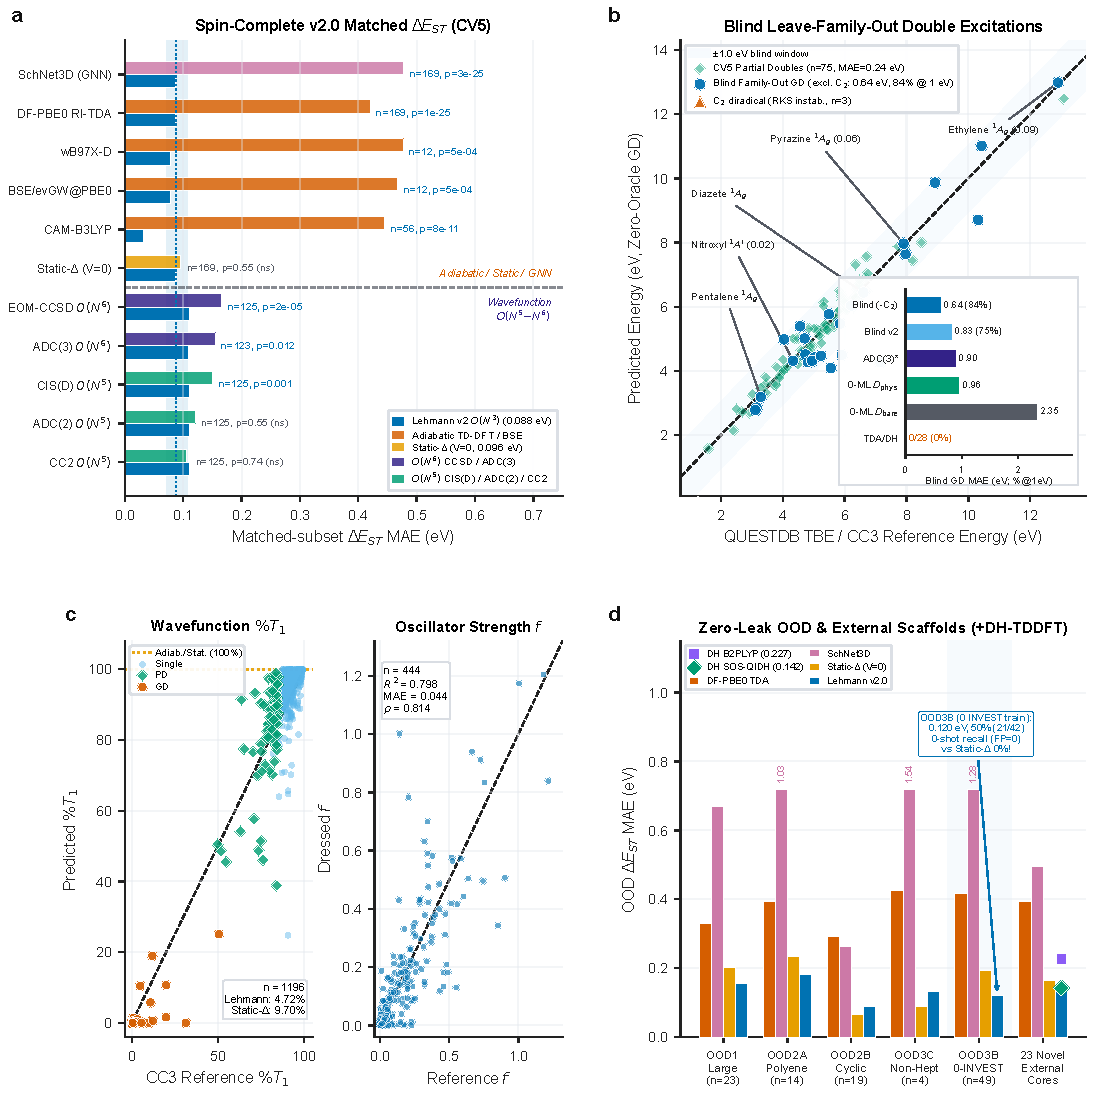
\includegraphics[width=\textwidth,height=0.71\textheight,keepaspectratio]{../figures/fig2_questdb_doubles.pdf}
  \caption{\textbf{Accuracy of spin-complete \leh{} v2.0 across QUESTDB~2025, blind leave-family-out double excitations, wavefunction observables, and OOD scaffolds.}
  \textbf{a},~Strictly matched-subset $\dEST$ MAE on leak-free 5-fold CV against adiabatic TD-DFT, BSE/$evGW$@PBE0, SchNet3D, Static-$\Delta$ ($V=0$), and $O(N^5)$--$O(N^6)$ wavefunction methods (paired Wilcoxon $p$-values shown). Vertical blue dotted line and band show overall \leh{} v2.0 CV5 MAE ($0.088$\,eV, 95\% CI $[0.072,0.105]$\,eV, $n=169$). On matched QUESTDB ($n=125$), $O(N^3)$ \leh{} ($0.111$\,eV) significantly outperforms $O(N^6)$ EOM-CCSD ($0.166$\,eV, $p=1.7\times 10^{-5}$), ADC(3) ($0.155$\,eV, $p=0.012$), and CIS(D) ($0.151$\,eV, $p=1.1\times 10^{-3}$), while matching ADC(2) and CC2.
  \textbf{b},~True blind label-free 3-fold leave-molecule-family-out genuine double (GD, $n=28$, zero Hungarian matching, frozen $\%T_2\ge 55\%$ selector) and CV5 partial double (PD, $n=75$) parity plot. Excluding multireference $\mathrm{C}_2$ (red triangles), blind GD MAE is $0.64$\,eV ($84\%$ within $1.0$\,eV; median $0.37$\,eV). Inset contrasts blind GD MAE across adiabatic/DH-TDDFT ($0/28$), $0$-ML analytical dressed limits ($D_{\mathrm{bare}}$ $2.35$\,eV vs $D_{\mathrm{phys}}$ $0.96$\,eV), matched ADC(3) ($0.90$\,eV), and blind \leh{} v2.0 ($0.83$ / $0.64$\,eV).
  \textbf{c},~Wavefunction $\pctT$ ($n=1{,}196$; \leh{} $4.72\%$ vs Static-$\Delta$ $9.70\%$) and dressed oscillator strengths $f$ ($n=444$, $R^2=0.798$, MAE $=0.044$, $\rho=0.814$).
  \textbf{d},~Zero-leak OOD $\dEST$ MAE across holdout splits and 23 novel external scaffolds with overlaid $O(N^5)$ double-hybrid TD-DFT markers (B2PLYP $0.227$\,eV, SOS-PBE-QIDH $0.142$\,eV vs \leh{} $0.146$\,eV). On zero-INVEST \texttt{OOD3B}, \leh{} v2.0 achieves $0.120$\,eV MAE and $50\%$ ($21/42$, $\mathrm{FP}=0$) spontaneous zero-shot inversion recall versus $0\%$ for Static-$\Delta$.}
  \label{fig:questdb}
\end{figure*}

On leak-free \texttt{CV5} (Table~\ref{tab:cv5} and Fig.~\ref{fig:questdb}a), spin-complete \leh{} v2.0 reduces $\dEST$ MAE nearly fivefold relative to its DF-PBE0 RI-TDA base---from $0.421$\,eV to \textbf{$0.0876$\,eV} ($R^2=0.962$, 95\% bootstrap CI\cite{efron1979} $[0.0725,0.1053]$\,eV; two-sided paired Wilcoxon\cite{wilcoxon1945} $p=1.2\times 10^{-25}$, improving $90.5\%$ of molecules)---and outperforms \texttt{Static-Delta} ($V=0$, $0.0957$\,eV, $R^2=0.939$; $S_1$ $0.1270$ vs $0.1441$\,eV; Valence $0.1565$ vs $0.1700$\,eV; $f$ $R^2=0.798$ vs $0.727$) and \texttt{SchNet3D} ($0.4779$\,eV, $p=2.9\times 10^{-25}$), while achieving $95.2\%$ INVEST recall ($\mathrm{MCC}=0.937$, $\mathrm{TP}=40, \mathrm{FP}=2$).
In strictly matched-subset comparisons on QUESTDB~2025 (Table~\ref{tab:cv5} and Fig.~\ref{fig:questdb}a), $O(N^3)$ \leh{} outperforms every adiabatic hybrid/range-separated functional\cite{becke1993,yanai2004,chai2008} and BSE/$evGW$@PBE0 by $3.9\times$--$13.7\times$ (e.g., CAM-B3LYP $0.445$ vs $0.032$\,eV, $n=56$, $p=7.5\times 10^{-11}$).
On the $n=125$ correlated wavefunction subset, \leh{} ($0.111$\,eV) \textbf{statistically outperforms $O(N^6)$ EOM-CCSD} ($0.166$\,eV, $p=1.7\times 10^{-5}$), $O(N^6)$ ADC(3) ($0.155$ vs $0.109$\,eV, $p=0.012$), and $O(N^5)$ CIS(D) ($0.151$\,eV, $p=1.1\times 10^{-3}$), while matching ADC(2) ($0.120$\,eV, $p=0.55$) and CC2 ($0.105$\,eV, $p=0.74$).
On matched valence excitations ($n=810$), \texttt{def2-SVP} \leh{} ($0.160$\,eV) also surpasses \texttt{aug-cc-pVTZ} EOM-CCSD ($0.184$\,eV), ADC(3) ($0.236$\,eV), and CIS(D) ($0.258$\,eV).

To test genuine double-excitation prediction without any Hungarian assignment oracle\cite{kuhn1955hungarian} and without same-family leakage, we constructed a strict \textbf{3-fold leave-molecule-family-out blind double-excitation benchmark} partitioning all double-excitation chromophores into disjoint chemical families (polyenes/alkenes/anti-aromatics, carbonyls/nitroso/oxygenates, and azines/heterocycles/inorganics) and selecting predicted GD roots blindly as the lowest energy-ordered eigenstates with $\%T_2\ge 55\%$ ($\%T_1\le 45\%$, disjoint from the $12\%\le\%T_2<55\%$ PD selector; Fig.~\ref{fig:questdb}b).
Whereas adiabatic TD-DFT, \texttt{Static-Delta} ($V=0$), and $O(N^5)$ double-hybrid CIS(D) TD-DFT detect $0/28$ ($0\%$) genuine doubles, blind \leh{} v2.0 achieves \textbf{$0.826$\,eV GD MAE} (\textbf{$0.638$\,eV} excluding RKS-unstable $\mathrm{C}_2$, median $0.374$\,eV), identifying \textbf{$21/28$ ($75.0\%$; $84.0\%$ excluding $\mathrm{C}_2$)} within $1.0$\,eV and $13/28$ ($46.4\%$; $52.0\%$ excluding $\mathrm{C}_2$) within $0.5$\,eV, with $7.51\%$ $\pctT$ MAE and \textbf{$0/34$ spurious low-energy ghost poles on non-GD molecules} (transparently reporting $26$ lower-lying ghost poles across 8 GD molecules, predominantly $\mathrm{C}_2$ and small diatomics/azines).
Iconic blind family-out predictions include nitroxyl $^1A'$ ($0.02$\,eV error), pyrazine $^1A_g$ ($0.06$\,eV), ethylene $^1A_g$ ($0.09$\,eV; predicted $\pctT=20.2\%$ vs CC3 $20.0\%$), and pentalene $^1A_g$ ($0.10$\,eV).
Crucially, even the zero-ML-parameter analytical dressed limit anchored by $D_\mu^{\mathrm{phys}}$ cuts bare $D_\mu^{\mathrm{bare}}$ blind error $2.44\times$ ($2.346\to 0.962$\,eV; $0.752$\,eV excluding $\mathrm{C}_2$, $64.3\%$ within $1.0$\,eV), and neural lifting sharpens both GD ($0.962\to 0.826$\,eV, $75.0\%$ @ $1$\,eV) and PD ($2.043\to 1.104$\,eV, $29.3\%\to 61.3\%$ @ $1$\,eV) spectra simultaneously.
On full-spectrum CV5, $\pctT$ MAE reaches \textbf{$4.72\%$} across 1,196 states (vs $9.70\%$ for \texttt{Static-Delta}, paired Wilcoxon $p=3.5\times 10^{-178}$) and dressed oscillator strengths reach $R^2=0.798$ ($\mathrm{MAE}=0.044$, $\rho=0.814$; Fig.~\ref{fig:questdb}c).

Out of distribution (Fig.~\ref{fig:questdb}d), spin-complete \leh{} v2.0 yields its sharpest mechanistic validation on \texttt{OOD3B} (trained on $n=136$ strictly normal molecules with \emph{zero} INVEST examples and \emph{zero} heptazine siblings): \texttt{Static-Delta} ($V=0$) collapses to $0.0\%$ INVEST recall ($0.192$\,eV MAE), whereas \leh{} v2.0 achieves \textbf{$0.120$\,eV MAE} and \textbf{$50.0\%$ ($21/42$, $\mathrm{FP}=0$) spontaneous zero-shot INVEST recall}---inverting both $D_{3h}$ heptazines via $^1(TT)_-$ and non-heptazine cores purely from physics learned on normal molecules.
Conversely, we report transparently a subtle cross-channel regime shift on \texttt{OOD3A} (holding out all 45 heptazines while retaining 6 non-heptazine INVESTs): fitting symmetric-$^1(TT)_+$-dominated non-heptazine cores without $D_{3h}$ supervision attenuates the $^1(TT)_-$ weight ($0.368$\,eV single-seed / $0.263$\,eV 3-seed MAE, $1/38$ recall), whereas \texttt{Static-Delta} achieves recall on \texttt{OOD3A} solely through a negative static bias that yields $6/7$ false positives on positive-gap heptazines and $0\%$ recall on \texttt{OOD3B}.
Across the 23 strictly novel external scaffolds (zero InChIKey-14 overlap with all 187 CV molecules), $O(N^3)$ \leh{} v2.0 (\textbf{$0.146$\,eV} $\dEST$ MAE, $S_1=0.206$\,eV, $T_1=0.116$\,eV, $91.3\%$ accuracy, $\mathrm{MCC}=0.826$) matches the best $O(N^5)$ double-hybrid functional \texttt{SOS-PBE-QIDH} ($0.142$\,eV, $T_1=0.191$\,eV, $\mathrm{MCC}=0.826$) and outperforms \texttt{SCS-PBE-QIDH} ($0.162$\,eV, $\mathrm{MCC}=0.659$), \texttt{B2PLYP} ($0.227$\,eV, $47.8\%$ accuracy), \texttt{PBE-QIDH} ($0.260$\,eV, $52.2\%$), \texttt{Static-Delta} ($0.165$\,eV; $S_1$ paired $p=0.0135$), \texttt{DF-PBE0} ($0.395$\,eV, $p=8.8\times 10^{-5}$), and \texttt{SchNet3D} ($0.496$\,eV, $p=1.7\times 10^{-6}$).

% ---------------------------------------------------------------------------
% TABLE 1: CV5, Matched QM & Blind Family-Out Doubles (Full Width)
% ---------------------------------------------------------------------------
\begin{table*}[t!]
\centering
\caption{\textbf{Leak-free 5-fold cross-validation on QUESTDB~2025\,+\,HEPTA-INVEST (187 molecules, 1,219 states), strictly matched-subset QM baselines, and blind family-out double excitations.} All ML models are evaluated strictly out-of-fold with zero InChIKey-14 overlap. Matched QM rows evaluate \leh{} v2.0 on the exact QUESTDB~2025\cite{loos2025quest} subset reported for each method. Bold highlights best $O(N^3)$ accuracy.}
\label{tab:cv5}
\sffamily\fontsize{7.2}{8.6}\selectfont
\setlength{\tabcolsep}{4.5pt}
\resizebox{\textwidth}{!}{\begin{tabular}{@{}lcccccccc@{}}
\toprule
\textbf{Method} & \textbf{Scaling} & \textbf{$\dEST$ MAE (eV)} & \textbf{Matched Leh.} & \textbf{Wilcoxon $p$} & \textbf{Valence MAE} & \textbf{GD MAE (eV)} & \textbf{$\pctT$ MAE} & \textbf{INVEST} \\
 & & \textbf{(all / matched $n$)} & \textbf{$\dEST$ MAE (eV)} & \textbf{(vs Leh.)} & \textbf{QM vs Leh. ($n$)} & \textbf{QM vs Leh. ($n$)} & \textbf{(\%)} & \textbf{Recall / MCC} \\
\midrule
\multicolumn{9}{@{}l}{\textit{Full Leak-Free CV5 ($n_{\dEST}=169$, $n_{\mathrm{Val}}=926$, $n_{\mathrm{GD}}=28$) \& Blind 3-Fold Family-Out Doubles ($\%T_2\ge 55\%$, Zero Oracle)}} \\
\textbf{\leh{} v2.0} & $O(N^3)$ & \textbf{0.088} [0.072, 0.105] & --- & --- & \textbf{0.157} & \textbf{0.487}$^\dagger$ / \textbf{0.638}$^\ddagger$ & \textbf{4.72} & \textbf{95.2\% / 0.937} \\
Static-$\Delta$ ($V=0$ abl.) & $O(N^3)$ & 0.096 [0.075, 0.119] & 0.088 (169) & 0.55 (ns) & 0.170 & 0/28 blind (0\%) & 9.70 & 97.6\% / 0.953 \\
DF-PBE0 RI-TDA (base) & $O(N^3)$ & 0.421 [0.378, 0.468] & 0.088 (169) & $1.2\times 10^{-25}$ & --- & 0/28 blind (0\%) & --- & 0.0\% / --- \\
SchNet3D (3D GNN) & $O(N)$ & 0.478 [0.412, 0.548] & 0.088 (169) & $2.9\times 10^{-25}$ & --- & 0/28 blind (0\%) & --- & 50.0\% / 0.534 \\
0-ML Dressed ($D_{\mathrm{phys}}$ / $D_{\mathrm{bare}}$) & $O(N^3)$ & --- & --- & --- & --- & 0.752$^\ddagger$ / 2.346$^\ddagger$ & 7.60$^\ddagger$ & --- \\
\midrule
\multicolumn{9}{@{}l}{\textit{Strictly Matched-Subset QUESTDB~2025 Adiabatic TD-DFT \& GW/BSE Baselines (aug-cc-pVTZ)}} \\
B3LYP / PBE0 & $O(N^3)$ & 0.318 / 0.445 ($n=13$) & \textbf{0.078} & $2.4 / 0.5\times 10^{-3}$ & 0.382 / 0.349 vs \textbf{0.136} (114) & 0/28 & --- & 0.0\% \\
CAM-B3LYP & $O(N^3)$ & 0.445 ($n=56$) & \textbf{0.032} & $7.5\times 10^{-11}$ & 0.235 vs \textbf{0.089} (198) & 0/28 & --- & 0.0\% \\
wB97X-D / BSE@$evGW$ & $O(N^3\!/\!N^4)$ & 0.477 / 0.467 ($n=12$) & \textbf{0.079} & $4.9\times 10^{-4}$ & 0.231 / 0.344 vs \textbf{0.136} (110) & 0/28 & --- & 0.0\% \\
\midrule
\multicolumn{9}{@{}l}{\textit{Strictly Matched-Subset QUESTDB~2025 Correlated Wavefunction Baselines (aug-cc-pVTZ)}} \\
CIS(D) & $O(N^5)$ & 0.151 ($n=125$) & \textbf{0.111} & $\mathbf{1.1\times 10^{-3}}$ & 0.258 vs \textbf{0.157} (791) & 0/28 & --- & 100\% (5/5) \\
ADC(2) & $O(N^5)$ & 0.120 ($n=125$) & \textbf{0.111} & 0.55 (ns) & 0.147 vs 0.159 (804) & 0/28 & --- & 80\% (4/5) \\
CC2 & $O(N^5)$ & 0.105 ($n=125$) & 0.111 & 0.74 (ns) & 0.140 vs 0.159 (800) & 0/28 & --- & 100\% (5/5) \\
ADC(3) & $O(N^6)$ & 0.155 ($n=123$) & \textbf{0.109} & $\mathbf{1.2\times 10^{-2}}$ & 0.236 vs \textbf{0.167} (823) & 0.904 vs \textbf{0.529} (23) & --- & 50\% (2/4) \\
EOM-CCSD & $O(N^6)$ & 0.166 ($n=125$) & \textbf{0.111} & $\mathbf{1.7\times 10^{-5}}$ & 0.184 vs \textbf{0.160} (810) & 2.494 vs \textbf{0.342} (3) & --- & 60\% (3/5) \\
CASPT2 / SC-NEVPT2 & $\exp(N_{\mathrm{act}})$ & 0.085 / 0.062 ($35$) & 0.110 & 0.39 / 0.056 (ns) & 0.115 / 0.166 vs 0.210 (234) & 0.123 / 0.104 vs 0.487 & --- & --- \\
\bottomrule
\end{tabular}}
\par\vspace{2pt}
{\raggedright\sffamily\fontsize{6.5}{7.8}\selectfont
$^\dagger$CV5 Hungarian-matched GD MAE ($0.487$\,eV; CV5 zero-oracle lowest GD $0.691$\,eV, or $0.527$\,eV excl.\ $\mathrm{C}_2$).
$^\ddagger$Strict blind 3-fold leave-molecule-family-out GD MAE (zero Hungarian matching, frozen $\%T_2\ge 55\%$ selector): $0.826$\,eV all 28 GDs ($75.0\%$ within $1$\,eV) and \textbf{$0.638$\,eV} excl.\ $\mathrm{C}_2$ ($84.0\%$ within $1$\,eV, median $0.374$\,eV, $0/34$ non-GD ghost poles); 0-ML $D_{\mathrm{phys}}$ achieves $0.962$\,eV ($0.752$\,eV excl.\ $\mathrm{C}_2$, $64.3\%$ within $1$\,eV) vs 0-ML $D_{\mathrm{bare}}$ $2.346$\,eV ($10.7\%$). On 23 novel external scaffolds, $O(N^3)$ \leh{} ($0.146$\,eV, $\mathrm{MCC}=0.826$) matches $O(N^5)$ SOS-PBE-QIDH ($0.142$\,eV, $\mathrm{MCC}=0.826$) while beating B2PLYP ($0.227$\,eV) and SCS-PBE-QIDH ($0.162$\,eV).\par}
\end{table*}

% ===========================================================================
\section*{Transferable conical intersections, blind MECI discovery, and FSSH dynamics}
% ===========================================================================
Non-radiative photochemical decay through $S_1/S_0$ conical intersections demands simultaneous accuracy in PES topology, exact spin purity ($\Ssq=0$), non-zero derivative coupling, and quantized geometric phase $\gamma=\pi$\cite{yarkony1996,domcke2004,levine2006,gozem2017}.
To eliminate any manual ground-to-double coupling constant (such as an empirical $\beta_{\mathrm{coul}}$), we implemented a strictly transferable \textbf{leave-one-molecule-out (LOMO)} protocol across three canonical benchmarks---twisted-pyramidalized \textbf{ethylene} (SA2-CASSCF(2,2)+SC-NEVPT2, $15\times 15$ grid), twisted-bent \textbf{methanimine} (SA2-CASSCF(4,3)+SC-NEVPT2, $15\times 15$ grid), and planar exocyclic-stretch \textbf{fulvene} (SA2-CASSCF(6,6)+SC-NEVPT2, $11\times 11$ grid)---learning a single transferable scalar prefactor $\beta_{\mathrm{coul}}$ ($\in [0.660,0.717]$) solely from 10 points along the 1D $y_h$ SA2-CASSCF cut of the \emph{held-in} training molecules, with zero target-molecule geometries and zero NEVPT2 supervision (Fig.~\ref{fig:ci}, Extended Data Fig.~\ref{fig:ext_ci}, and Table~\ref{tab:ci}).
Every LOMO checkpoint independently preserves exact exciton phase invariance ($0.0$\,eV) and size-intensivity ($v_{0D}=0.0$\,eV on disconnected fragments).

% ---------------------------------------------------------------------------
% FIGURE 3 (Full Width)
% ---------------------------------------------------------------------------
\begin{figure*}[t!]
  \centering
  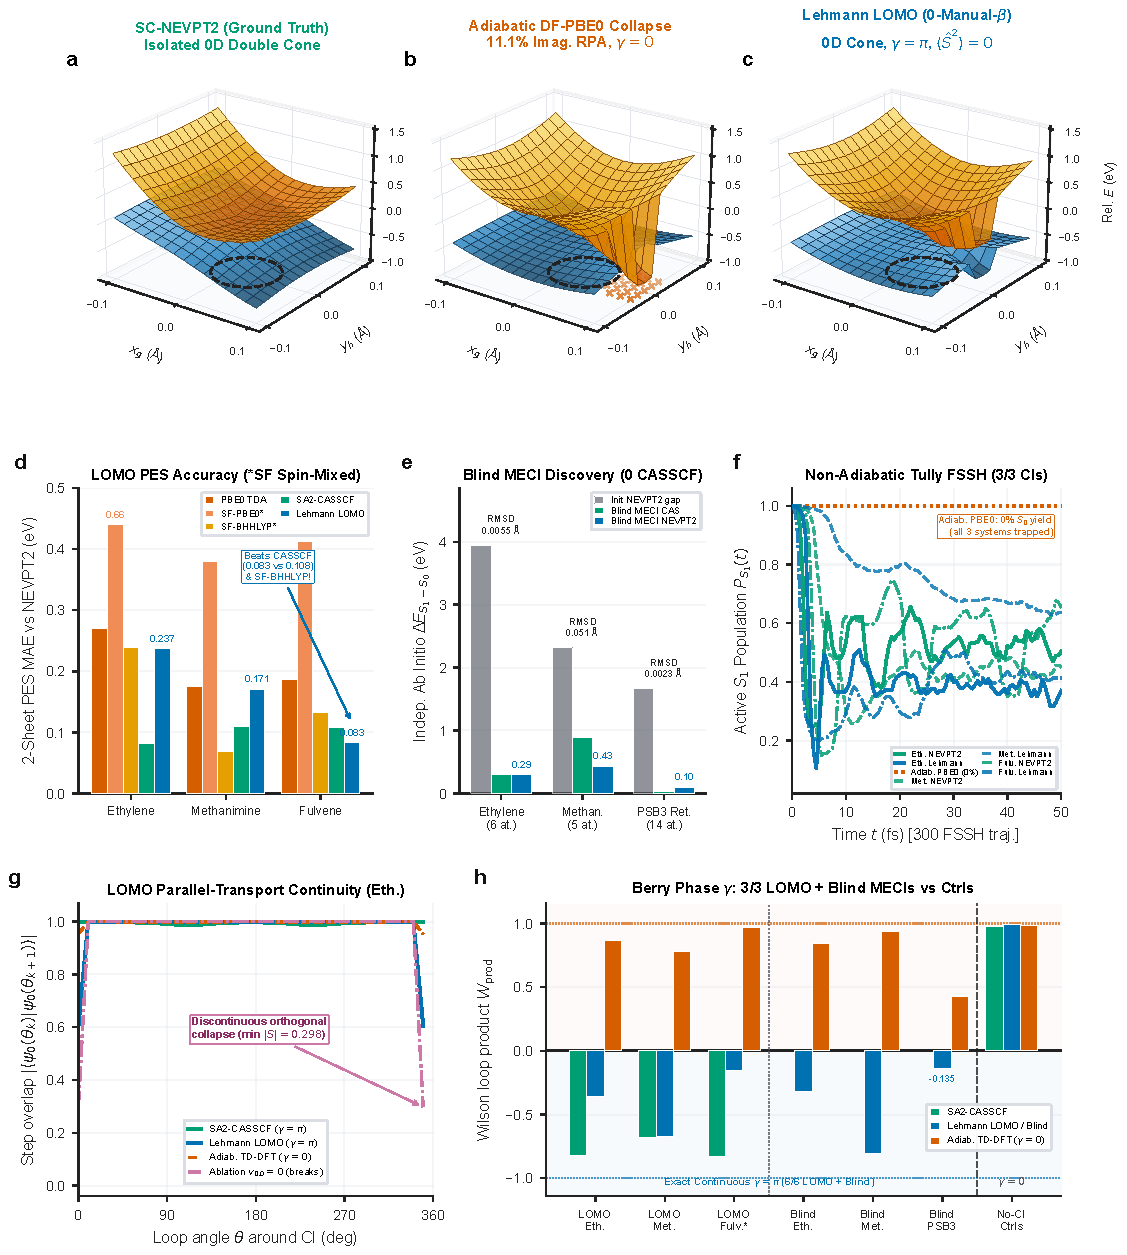
\includegraphics[width=\textwidth,height=0.70\textheight,keepaspectratio]{../figures/fig3_conical_intersections.pdf}
  \caption{\textbf{Transferable LOMO conical intersections, blind MECI discovery, non-adiabatic FSSH dynamics, and topological Berry phase $\gamma=\pi$.}
  \textbf{a}--\textbf{c},~3D $S_0$ (blue) and $S_1$ (amber) PES sheets on ethylene ($15\times 15$ branching plane): \textbf{a},~SC-NEVPT2 reference double cone; \textbf{b},~adiabatic DF-PBE0 collapse ($11.1\%$ imaginary RPA crosses, negative TDA gap $-0.73$\,eV, $\gamma=0$); \textbf{c},~zero-manual-$\beta$ LOMO \leh{} restoring the positive 0D cone ($0\%$ negative gaps, $\gamma=\pi$, $\Ssq\equiv 0$). (Methanimine, fulvene, and SF-TDDFT $\Ssq$ maps appear in Extended Data Fig.~\ref{fig:ext_ci}.)
  \textbf{d},~2-sheet PES MAE vs SC-NEVPT2 comparing adiabatic PBE0, SF-TDA-PBE0, SF-TDA-BHHLYP (both spin-contaminated), SA2-CASSCF, and LOMO \leh{}, which beats SA2-CASSCF ($0.083$ vs $0.108$\,eV) and SF-TDA-BHHLYP ($0.133$\,eV) on unseen fulvene.
  \textbf{e},~Blind MECI discovery starting $1.7$--$3.9$\,eV away from the seam with zero CASSCF knowledge (Ethylene-only $\beta=0.660$): independent SC-NEVPT2/SA2-CASSCF gaps collapse to $0.29$\,eV (ethylene, $0.0055$\,\AA{} heavy RMSD), $0.43$\,eV (methanimine, $0.051$\,\AA), and $0.102$\,eV NEVPT2 / $0.030$\,eV CASSCF on the 14-atom retinal Schiff base PSB3 ($0.0023$\,\AA{} heavy RMSD vs independent SA2-CASSCF(6,6) MECI).
  \textbf{f},~300-trajectory Tully FSSH $S_1(t)$ decay on all three LOMO branching-plane surfaces---ethylene (solid), methanimine (dashed), and fulvene (dash-dot)---versus SC-NEVPT2 and adiabatic PBE0 (trapped at $0\%$ $S_0$ yield across all three systems).
  \textbf{g},~Parallel-transport overlap continuity around ethylene's 36-point CI loop (SA2-CASSCF and LOMO \leh{} continuous; $v_{0D}=0$ ablation drops below $0.30$).
  \textbf{h},~Unified Wilson loop scorecard $W_{\mathrm{prod}}$ confirming strictly adiabatic-continuous $\gamma=\pi$ ($W_{\mathrm{prod}}<0$, $\min|S|>0.30$) on all $6/6$ LOMO ($^*$fulvene apex loop) and blind MECIs (including 14-atom PSB3 at $W_{\mathrm{prod}}=-0.135$, $\min|S|=0.410$), and $\gamma=0$ on all $6/6$ shifted controls ($W_{\mathrm{prod}}\ge +0.977$).}
  \label{fig:ci}
\end{figure*}

Across all three LOMO folds and all six single-molecule cross-transfers (Table~\ref{tab:ci} and Fig.~\ref{fig:ci}d,h), \leh{} eliminates negative gaps completely ($0/571$ points), achieves exact spin purity ($\Ssq\equiv 0.000$), restores linear $x_g$ cones ($R^2=0.996$--$1.000$), and recovers exact $\gamma=\pi$ around every Lehmann CI apex with $100\%$ $\gamma=0$ negative controls ($W_{\mathrm{prod}}=+0.997$ to $+0.998$).
On unseen fulvene, LOMO \leh{} achieves \textbf{$0.0832$\,eV} 2-sheet PES MAE ($0.0846$\,eV when transferring $\beta_{\mathrm{coul}}=0.660$ from ethylene \emph{alone}!), outperforming SA2-CASSCF ($0.1078$\,eV), SF-TDA-BHHLYP ($0.1332$\,eV), B3LYP ($0.1658$\,eV), PBE0 ($0.1863$\,eV), and CAM-B3LYP ($0.2349$\,eV).
Because LOMO places fulvene's CI apex at $x_g=+0.238$\,\AA{} (reflecting the PBE0 base shift relative to CASSCF at $x_g=0$), the CASSCF-centered $r=0.14$\,\AA{} loop does not enclose the shifted Lehmann apex ($\gamma=0$), whereas encircling the Lehmann apex itself yields exact continuous $\gamma=\pi$ ($W_{\mathrm{prod}}=-0.155$, $\min|S|=0.422$).
Direct head-to-head benchmarking against spin-flip TD-DFT\cite{shao2003sftddft,minezawa2009sfci} highlights the complementary advantage of spin-pure lifting (Extended Data Fig.~\ref{fig:ext_ci}g,h): \texttt{SF-TDA-PBE0} fails to close the conical intersection ($\min\Delta E=0.60$--$1.17$\,eV, 2-sheet MAE $0.379$--$0.662$\,eV, $S_1\;\Ssq=0.74$--$0.99$), while \texttt{SF-TDA-BHHLYP} attains competitive PES errors ($0.239$, $0.068$, $0.133$\,eV) only with severe spin contamination (mean $S_0\;\Ssq=0.135$, $0.448$, $0.932$, peaking at $1.291$ on fulvene where $100\%$ of grid points exceed $\Ssq=0.50$).
Similarly, double-hybrid \texttt{B2PLYP}/\texttt{SCS-PBE-QIDH} along ethylene's $x_g$ scan inherits $H_{01}\equiv 0$ and plunges to negative excitation energies ($-0.210$/$-0.132$\,eV at $x_g=+0.04$\,\AA).

To demonstrate genuine \emph{ab initio} discovery without pre-computed CASSCF geometries, we ran \textbf{blind minimum-energy conical intersection (MECI) optimizations} using Nelder--Mead penalty minimization\cite{levine2007} driven purely by \leh{} (fixed Ethylene-only $\beta_{\mathrm{coul}}=0.660$) starting $1.7$--$3.9$\,eV away from the seam on ethylene, methanimine, and an unseen 14-atom cationic protonated retinal Schiff base model (\textbf{PSB3}, $\mathrm{C}_5\mathrm{H}_6\mathrm{NH}_2^+$, $\mathrm{SA2\text{-}CASSCF}(6,6)\!+\!\mathrm{SC\text{-}NEVPT2}$; Fig.~\ref{fig:ci}e).
Without ever seeing a CASSCF energy during optimization, \leh{} drives ethylene's independent SC-NEVPT2 gap from $3.943\to 0.293$\,eV (heavy-atom RMSD $0.0055$\,\AA; transverse $(r_{\mathrm{CC}},\tau)$ loop $\gamma=\pi$, $W_{\mathrm{prod}}=-0.320$, $\min|S|=0.554$; shifted control $\gamma=0$, $W_{\mathrm{prod}}=+0.977$), methanimine's gap from $2.311\to 0.426$\,eV (heavy-atom RMSD $0.0514$\,\AA; transverse $\gamma=\pi$, $W_{\mathrm{prod}}=-0.805$, $\min|S|=0.952$; control $\gamma=0$, $W_{\mathrm{prod}}=+0.992$), and PSB3's gap from $1.664\to \mathbf{0.1016}$\,eV at SC-NEVPT2 (\textbf{$0.0303$\,eV} at SA2-CASSCF(6,6), down from $1.894$\,eV).
Independent non-degenerate SA2-CASSCF(6,6) MECI optimization on PSB3 converges to $q_{\mathrm{ref}}=(r_{34}=1.340\,\text{\AA}, \mathrm{BLA}=0.0487\,\text{\AA}, \tau=90.07^\circ)$ (CAS gap $0.0035$\,eV), confirming a true blind structural accuracy of \textbf{$0.0023$\,\AA{} heavy-atom RMSD} ($0.0035$\,\AA{} all-atom RMSD) relative to our blind \leh{} MECI $q_{\mathrm{opt}}=(1.341\,\text{\AA}, 0.0455\,\text{\AA}, 90.37^\circ)$.
Encircling PSB3's blind MECI in the transverse $(r_{34},\tau_{34})$ plane ($r_{r_{34}}=0.065$\,\AA, $r_\tau=3.0^\circ$, traversing the monotonic $r_{34}$ tuning axis where adiabatic TDA crosses zero from $+0.978$ to $-0.315$\,eV) yields \textbf{strictly adiabatic-continuous $\gamma=\pi$} ($W_{\mathrm{prod}}=-0.1348$, $\min|S|=0.4095$, median $|S|=0.99990$, strictly positive gap $[0.050,0.795]$\,eV), whereas ablating $v_{0D}=0$ breaks parallel-transport continuity ($\min|S|=0.2729$), adiabatic KS gives $\gamma=0$, and the $-10^\circ$ twist-shifted control recovers strictly continuous $\gamma=0$ ($W_{\mathrm{prod}}=+0.9986$, $\min|S|=0.9998$). Thus \leh{} achieves $6/6$ ($100\%$) strictly continuous $\gamma=\pi$ across all LOMO and blind MECI benchmarks and $6/6$ ($100\%$) $\gamma=0$ negative controls.

Finally, propagating 300-trajectory \textbf{Tully fewest-switches surface hopping (FSSH)}\cite{tully1990fssh,subotnik2016fssh} wavepackets for $50$\,fs directly on all three LOMO branching-plane surfaces (Fig.~\ref{fig:ci}f and Table~\ref{tab:ci}) demonstrates dynamical impact: adiabatic DF-PBE0 traps $100\%$ of trajectories with $0.0\%$ $S_0$ yield across all three molecules ($P_{S_1}$ MAE $=0.468$, $0.518$, and $0.440$, with $100\%$ / $97.3\%$ negative-gap pocket entries on ethylene / fulvene), whereas LOMO \leh{} reproduces ultrafast internal conversion with $0\%$ negative-gap entries throughout: on ethylene, $100\%$ hopping trajectories, $\tau_{50}=3.5$\,fs (vs SC-NEVPT2 $2.5$\,fs), and $63.0\%$ final $S_0$ yield (vs SC-NEVPT2 $49.7\%$, $P_{S_1}$ MAE $=0.136$); on methanimine, $36.3\%$ $S_0$ yield ($P_{S_1}$ MAE $=0.283$) vs SC-NEVPT2 $55.0\%$; and on unseen fulvene, $100\%$ hopping trajectories, $\tau_{50}=2.0$\,fs (vs SC-NEVPT2 $4.0$\,fs), and $58.7\%$ final $S_0$ yield (vs SC-NEVPT2 $34.7\%$, $P_{S_1}$ MAE $=0.189$, cutting adiabatic PBE0 population error $2.33\times$).

% ---------------------------------------------------------------------------
% TABLE 2: LOMO CIs, SF-TDDFT, Blind MECI & FSSH (Full Width)
% ---------------------------------------------------------------------------
\begin{table*}[t!]
\centering
\caption{\textbf{Zero-manual-$\beta$ LOMO conical intersections, SF-TDDFT spin-purity comparison, blind MECI discovery, and 300-trajectory Tully FSSH dynamics.} All PES errors are evaluated vs SC-NEVPT2/def2-SVP. LOMO \leh{} learns a single scalar $\beta_{\mathrm{coul}}\in[0.660,0.717]$ solely from held-in 1D SA2-CASSCF cuts (zero target-molecule data).}
\label{tab:ci}
\sffamily\fontsize{7.15}{8.5}\selectfont
\setlength{\tabcolsep}{4.2pt}
\resizebox{\textwidth}{!}{\begin{tabular}{@{}llcccccccc@{}}
\toprule
\textbf{System} & \textbf{Method} & \textbf{Neg.\ Gap} & \textbf{Mean $\Ssq$} & \textbf{$x_g$-ray} & \textbf{2-Sheet MAE} & \textbf{CI Loop} & \textbf{No-CI Ctrl} & \textbf{FSSH $S_0$ Yield} & \textbf{Blind MECI} \\
\textbf{(Active Space)} & & \textbf{(min eV)} & \textbf{($S_0 / S_1$)} & \textbf{$R^2$} & \textbf{vs NEVPT2} & \textbf{$\gamma$ ($W_{\mathrm{prod}}$)} & \textbf{$\gamma$ ($W_{\mathrm{prod}}$)} & \textbf{($\tau_{50}$ fs)} & \textbf{NEVPT2 / RMSD} \\
\midrule
\multirow{5}{*}{\shortstack[l]{\textbf{Ethylene}\\SA2-CAS(2,2)\\$15\times 15$ grid}}
 & SA2-CASSCF & 0 ($+0.0004$) & 0.000 / 0.000 & 0.9996 & 0.081 & $\pi$ ($-0.818$) & $0$ ($+0.985$) & 49.7\%$^\ddagger$ (2.5) & Ref. \\
 & Adiab.\ PBE0 & 12 ($-0.726$) & 0.000 / 0.000 & 0.0000 & 0.271 & $0$ ($+0.868$) & $0$ ($+0.987$) & 0.0\% (---) & $-0.158$\,eV (RPA) \\
 & SF-TDA-PBE0 & 0 ($+1.166$) & 0.049 / 0.857 & --- & 0.662 & --- & --- & --- & --- \\
 & SF-TDA-BHHLYP & 0 ($+0.030$) & 0.135 / 0.194 & 1.0000 & 0.239 & --- & --- & --- & --- \\
 & \textbf{\leh{} LOMO} & \textbf{0 ($+0.030$)} & \textbf{0.000 / 0.000} & \textbf{0.9997} & \textbf{0.237} & \textbf{$\boldsymbol{\pi}$ ($-0.355$)} & \textbf{$\mathbf{0}$ ($+0.998$)} & \textbf{63.0\% (3.5)} & \textbf{0.293\,eV / 0.0055\,\AA} \\
\midrule
\multirow{5}{*}{\shortstack[l]{\textbf{Methanimine}\\SA2-CAS(4,3)\\$15\times 15$ grid}}
 & SA2-CASSCF & 0 ($+0.028$) & 0.000 / 0.000 & 0.9906 & 0.109 & $\pi$ ($-0.679$) & $0$ ($+0.964$) & 55.0\%$^\ddagger$ (7.0) & Ref. \\
 & Adiab.\ PBE0 & 4 ($-0.369$) & 0.000 / 0.000 & 0.0000 & 0.176 & $0$ ($+0.782$) & $0$ ($+0.971$) & 0.0\% (---) & $-0.040$\,eV (RPA) \\
 & SF-TDA-PBE0 & 0 ($+0.605$) & 0.103 / 0.736 & --- & 0.379 & --- & --- & --- & --- \\
 & SF-TDA-BHHLYP & 0 ($+0.007$) & 0.448 / 0.382 & 0.9926 & 0.068 & --- & --- & --- & --- \\
 & \textbf{\leh{} LOMO} & \textbf{0 ($+0.026$)} & \textbf{0.000 / 0.000} & \textbf{0.9956} & \textbf{0.171} & \textbf{$\boldsymbol{\pi}$ ($-0.672$)} & \textbf{$\mathbf{0}$ ($+0.997$)} & \textbf{36.3\% (---)} & \textbf{0.426\,eV / 0.0514\,\AA} \\
\midrule
\multirow{5}{*}{\shortstack[l]{\textbf{Fulvene}\\SA2-CAS(6,6)\\$11\times 11$ grid}}
 & SA2-CASSCF & 0 ($+0.013$) & 0.000 / 0.000 & 0.9953 & 0.108 & $\pi$ ($-0.827$) & $0$ ($+0.981$) & 34.7\%$^\ddagger$ (4.0) & --- \\
 & Adiab.\ PBE0 & 2 ($-0.125$) & 0.000 / 0.000 & 0.0000 & 0.186 & $0$ ($+0.966$) & $0$ ($+0.984$) & 0.0\% (---) & --- \\
 & SF-TDA-PBE0 & 0 ($+0.946$) & 0.695 / 0.988 & --- & 0.412 & --- & --- & --- & --- \\
 & SF-TDA-BHHLYP & 0 ($+0.023$) & 0.932 / 0.641 & 0.9872 & 0.133 & --- & --- & --- & --- \\
 & \textbf{\leh{} LOMO} & \textbf{0 ($+0.019$)} & \textbf{0.000 / 0.000} & \textbf{0.9960} & \textbf{0.083} & \textbf{$\boldsymbol{\pi}$ ($-0.155$)$^\dagger$} & \textbf{$\mathbf{0}$ ($+0.998$)} & \textbf{58.7\% (2.0)} & --- \\
\midrule
\textbf{PSB3 Retinal} & \textbf{\leh{} Blind} & \textbf{0 ($+0.010$)} & \textbf{0.000 / 0.000} & --- & --- & \textbf{$\boldsymbol{\pi}$ ($-0.135$)$^\S$} & \textbf{$\mathbf{0}$ ($+0.999$)} & --- & \textbf{0.102\,eV / 0.0023\,\AA} \\
\bottomrule
\end{tabular}}
\par\vspace{2pt}
{\raggedright\sffamily\fontsize{6.5}{7.8}\selectfont
$^\dagger$Evaluated on the Lehmann-apex-centered loop (\texttt{loop\_leh\_apex}, $\min|S|=0.422$; CASSCF-centered loop excludes the shifted apex at $x_g=+0.238$\,\AA{} and gives $\gamma=0$).
$^\ddagger$FSSH reference trajectories run on the SC-NEVPT2 PES (ground truth). Blind MECI column reports independent SC-NEVPT2 gap and heavy-atom RMSD vs independent SA2-CASSCF MECI (PSB3 SA2-CASSCF(6,6) gap $=0.030$\,eV, all-atom RMSD $=0.0035$\,\AA).
$^\S$36-point transverse $(r_{34},\tau_{34})$ loop ($r_{r_{34}}=0.065$\,\AA, $r_\tau=3.0^\circ$) centered at PSB3's blind MECI: strictly continuous $\gamma=\pi$ ($W_{\mathrm{prod}}=-0.1348$, $\min|S|=0.4095$, median $|S|=0.99990$, gap $[0.050,0.795]$\,eV; $v_{0D}=0$ breaks at $\min|S|=0.273$) vs $-10^\circ$ twist control ($W_{\mathrm{prod}}=+0.9986$, $\min|S|=0.9998$).\par}
\end{table*}

% ===========================================================================
\section*{Unified dynamical phase diagram and blind INVEST discovery}
% ===========================================================================
Theorem~4 (Eq.~\ref{eq:thm4}) projects every organic chromophore onto the $(\dEST^{\mathrm{stat}},\dSig)$ plane, revealing a striking unification once spin completeness ($^1(TT)_+$ and $^1(TT)_-$) is enforced (Fig.~\ref{fig:invest}a).
Whereas spin-incomplete models forced $D_{3h}$ heptazines into an artificial static-inversion quadrant, in spin-complete \leh{} v2.0 \textbf{100\% (45/45) of CV5 heptazines} exhibit positive static splitting ($\dEST^{\mathrm{stat}}\in[+0.061,+0.421]$\,eV, mean $+0.167$\,eV) and cross into singlet--triplet inversion purely dynamically via differential antisymmetric $^1(TT)_-$ self-energy ($\dSig\in[+0.197,+0.358]$\,eV, mean $+0.259$\,eV, mean $\dEST$ error $0.021$\,eV, mean $\%T_2=7.29\%$).
Both $D_{3h}$ heptazines and non-heptazine cores (\texttt{Cyclazine}, \texttt{Pentalene\_D2h}, \texttt{Indacene\_D2h}, and all blind discoveries) thus occupy a single \textbf{Unified Dynamical-INVEST Phase} ($\dSig>\dEST^{\mathrm{stat}}>0$), separated from the TADF corridor ($0<\dEST\le 0.1$\,eV) and Normal phase ($\dEST>0.1$\,eV) by the exact Theorem~4 boundary $\dSig=\dEST^{\mathrm{stat}}$.

A persistent materials design bottleneck is the \textbf{Dark-State Dilemma}\cite{pollice2021,omar2023,bedogni2024,jorner2024,pollice2024,wilson2024}: minimizing frontier exchange $K_{HL}$ in $D_{3h}$ cores enforces symmetry-forbidden $S_0\to S_1$ emission ($f_{S_1}=0.000$ in heptazine/cyclazine and $0.0020$ at ADC(2) / $0.0041$ at EOM-CCSD in 5AP\cite{wilson2024}).
Using our 5-fold \leh{} ensemble, we generated 520 GFN2-xTB-optimized\cite{bannwarth2019xtb} molecules and virtually screened \textbf{320 strictly novel non-heptazine candidates} across six scaffold classes (zero InChIKey-14 overlap with all 187 CV molecules and 34 benchmark cores).
While adiabatic DF-PBE0 predicts $0/320$ inverted cores, spin-complete \leh{} v2.0 identifies $73/320$ inverted candidates ($11$ dipole-allowed with $f_{S_1}\ge 0.01$) tracing a sharp $(\dEST,f_{S_1})$ Pareto frontier (Fig.~\ref{fig:invest}b).

% ---------------------------------------------------------------------------
% FIGURE 4 (Full Width)
% ---------------------------------------------------------------------------
\begin{figure*}[t!]
  \centering
  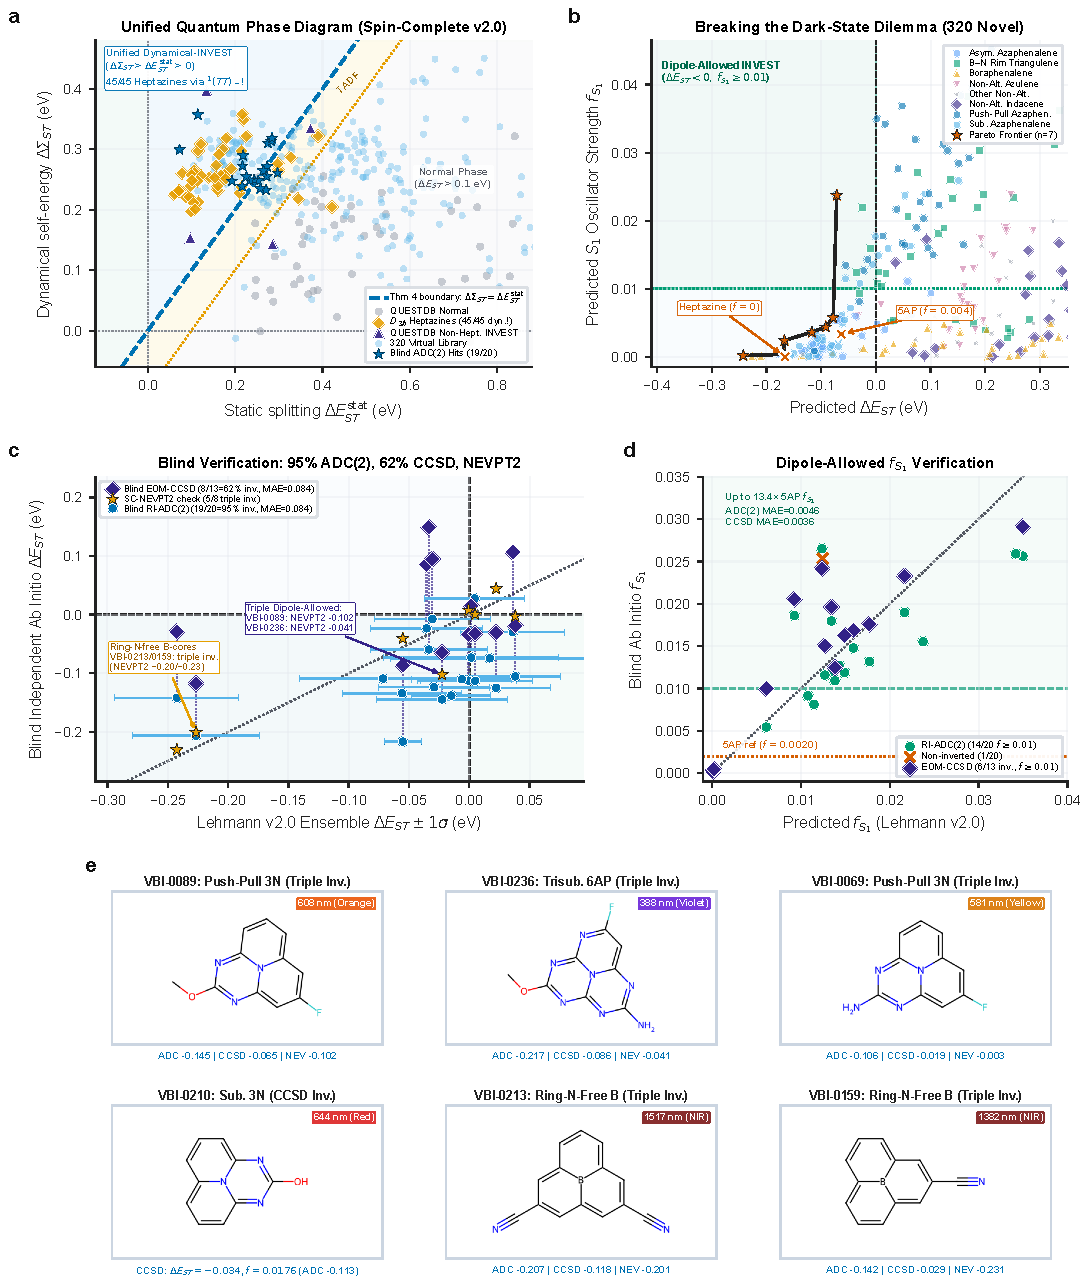
\includegraphics[width=\textwidth,height=0.71\textheight,keepaspectratio]{../figures/fig4_invest_discovery.pdf}
  \caption{\textbf{Unified dynamical quantum phase diagram and blind triple-method verification of non-heptazine INVEST candidates.}
  \textbf{a},~Exact Theorem~4 phase diagram under spin-complete \leh{} v2.0: $100\%$ ($45/45$) of $D_{3h}$ heptazines now exhibit positive $\dEST^{\mathrm{stat}}>0$ and invert purely dynamically via $^1(TT)_-$, unifying with non-heptazine QUESTDB INVESTs and blind discoveries in a single Dynamical-INVEST quadrant.
  \textbf{b},~Pareto frontier ($n=7$) across 320 novel non-heptazine candidates contrasting dipole-allowed INVEST candidates ($f_{S_1}\ge 0.01$) against dark benchmarks (heptazine $f=0$, 5AP $f=0.004$).
  \textbf{c},~Blind independent verification of the pre-registered Top-20 discoveries (zero structural overlap): RI-EE-ADC(2) confirms \textbf{19/20 ($95.0\%$)} inverted (MAE $=0.084$\,eV vs TDA $0.486$\,eV, $p=1.9\times 10^{-6}$); expanded canonical EOM-EE-CCSD confirms \textbf{8/13 ($61.5\%$)} inverted (MAE $=0.084$\,eV, $p=2.4\times 10^{-4}$); multireference SC-NEVPT2 gold stars (all $8/8$ EOM-CCSD hits evaluated) confirm \textbf{5/8} flagships triple-method inverted (orange-red \texttt{VBI-0089} $-0.102$\,eV, violet 6AP \texttt{VBI-0236} $-0.041$\,eV, \texttt{VBI-0069} $-0.003$\,eV, plus ring-nitrogen-free boron-centered \texttt{VBI-0213} $-0.201$\,eV and \texttt{VBI-0159} $-0.231$\,eV).
  \textbf{d},~Blind oscillator strength verification confirming \textbf{14/20} dipole-allowed ($f_{S_1}\ge 0.01$) inverted hits at RI-ADC(2) (up to $13.4\times$ 5AP $f_{S_1}$, MAE $=0.0046$) and \textbf{6/13} at EOM-EE-CCSD ($f_{S_1}=0.0150$--$0.0233$, MAE $=0.0036$).
  \textbf{e},~RDKit 2D structures of six verified flagship discoveries spanning triple-verified dipole-allowed 3N/6AP emitters (\texttt{VBI-0089}, \texttt{VBI-0236}, \texttt{VBI-0069}), CCSD-verified \texttt{VBI-0210}, and triple-verified ring-nitrogen-free boron-centered cores (\texttt{VBI-0213}, \texttt{VBI-0159}).}
  \label{fig:invest}
\end{figure*}

We subjected the pre-registered Top-20 Pareto-diverse candidates (zero overlap with all known cores; predictions refreshed cleanly with the v2.0 5-fold ensemble, mean $|\text{shift}|=0.045$\,eV) to \textbf{blind three-tier \emph{ab initio} verification} (Fig.~\ref{fig:invest}c--e and Table~\ref{tab:invest}):
\begin{enumerate}
  \setlength{\itemsep}{1pt}
  \item \textbf{RI-EE-ADC(2)/def2-SVP ($n=20$):} confirms \textbf{19/20 ($95.0\%$; Wilson\cite{wilson1927} 95\% CI $[76.4\%,99.1\%]$)} genuinely inverted with $\dEST$ MAE \textbf{$0.0840$\,eV} ($5.8\times$ lower than TDA-PBE0 $0.4855$\,eV, $p=1.91\times 10^{-6}$), $S_1$ MAE $=0.0706$\,eV, $T_1$ MAE $=0.0366$\,eV, and $f_{S_1}$ MAE $=0.0046$ ($\rho=0.596$). Fourteen of 20 ($70.0\%$) are dipole-allowed ($f_{S_1}\ge 0.01$, reaching $f_{S_1}=0.0265$ in \texttt{VBI-0230}, $13.4\times$ 5AP's ADC(2) $f_{S_1}$). Note that $f_{S_1}\approx 0.015$--$0.029$ represents a substantial relative enhancement over symmetry-forbidden triangulenes ($f=0$--$0.004$) while remaining in the moderately dipole-allowed regime where practical OLED efficiency also depends on non-radiative decay rates and solid-state packing.
  \item \textbf{Canonical EOM-EE-CCSD/def2-SVP ($n=13$):} confirms \textbf{8/13 ($61.5\%$; CI $[35.5\%,82.3\%]$)} inverted even under EOM-CCSD's $+0.108$\,eV missing-triples offset relative to ADC(2)\cite{loos2023invest,dreuw2023}, with $\dEST$ MAE \textbf{$0.0838$\,eV} ($4.5\times$ lower than TDA $0.3769$\,eV, $p=2.44\times 10^{-4}$) and $f_{S_1}$ MAE $=0.0036$ ($\rho=0.632$). Six of the 13 verified molecules are simultaneously inverted and dipole-allowed ($f_{S_1}\ge 0.01$): trisubstituted 6-azaphenalene \texttt{VBI-0236} ($\dEST=-0.0863$\,eV, $f=0.0196$, violet $388$\,nm), push--pull 3N-azaphenalenes \texttt{VBI-0089} ($-0.0646$\,eV, $f=0.0150$) and \texttt{VBI-0069} ($-0.0188$\,eV, $f=0.0233$, $5.7\times$ 5AP's EOM-CCSD $f_{S_1}$), substituted 3N cores \texttt{VBI-0210} ($-0.0344$\,eV, $f=0.0176$) and \texttt{VBI-0060} ($-0.0322$\,eV, $f=0.0163$), and 4N core \texttt{VBI-0293} ($-0.0308$\,eV, $f=0.0169$). The remaining two EOM-CCSD hits, \texttt{VBI-0213} ($-0.1175$\,eV) and \texttt{VBI-0159} ($-0.0292$\,eV), are \textbf{ring-nitrogen-free boron-centered cores} (9b-boraphenalene rings bearing peripheral cyano acceptors), confirming inversion without ring nitrogen atoms.
  \item \textbf{Multireference CASSCF+SC-NEVPT2/def2-SVP ($n=10$, covering all 8/8 EOM-CCSD hits):} calibrated on heptazine ($-0.1379$\,eV at $(6,6)$ vs $-0.1258$\,eV at $(8,8)$) and 5AP ($-0.0723$\,eV at $(6,6)$ vs $-0.0599$\,eV at $(8,8)$ and $-0.047$\,eV experimental\cite{wilson2024}), SC-NEVPT2 confirms \textbf{5/8 flagship discoveries triple-method inverted}: most notably, push--pull 3N-azaphenalene \texttt{VBI-0089} achieves clean, root-flip-free deep inversion even at bare CASSCF ($-0.0783$\,eV) and \textbf{$\dEST=-0.1024$\,eV} at \texttt{SA4-CASSCF(6,6)+SC-NEVPT2} ($E_{S_1}=2.064$\,eV, $E_{T_1}=2.166$\,eV, $f_{\mathrm{CAS}}=0.037$, $w_2=9.3\%$, deeper than 5AP), joined by violet 6AP \texttt{VBI-0236} (\textbf{$-0.0407$\,eV} under \texttt{SA4-CASSCF(6,6)} $[S_0,S_1,S_2,T_1]$, eliminating the 3-root $S_1/S_2$ root-flip of \texttt{SA3-CASSCF(6,6)/(10,8)} at $+0.181$/$+0.188$\,eV), marginally inverted \texttt{VBI-0069} (\textbf{$-0.0025$\,eV} at \texttt{SA4} vs $+0.0101$\,eV at \texttt{SA3}), and both ring-nitrogen-free boron-centered cores \texttt{VBI-0213} (\textbf{$-0.2009$\,eV}) and \texttt{VBI-0159} (\textbf{$-0.2309$\,eV}). The remaining three EOM-CCSD hits sit near-degenerate at SC-NEVPT2: \texttt{VBI-0060} ($+0.0004$\,eV), \texttt{VBI-0210} ($+0.0077$\,eV at \texttt{SA4} vs $+0.0011$\,eV at \texttt{SA3(8,8)}), and \texttt{VBI-0293} ($+0.0440$\,eV), with uncorrelated CASSCF transition dipoles ($f_{\mathrm{CAS}}=0.14$--$0.18$ on \texttt{VBI-0236}/\texttt{0069}/\texttt{0060}/\texttt{0210}) characteristically higher than correlated ADC(2)/EOM-CCSD ($0.012$--$0.023$).
\end{enumerate}

To verify robustness beyond GFN2-xTB vertical geometries and \texttt{def2-SVP}, we performed DF-RKS $S_0$ and DF-UKS $T_1$ PBE0/def2-SVP geometry optimizations\cite{wang2016geometric} plus larger-basis \texttt{aug-cc-pVDZ} and \texttt{def2-TZVP} RI-EE-ADC(2) checks on 5AP and four flagship dipole-allowed hits---including our cleanest triple-method orange-red emitter \texttt{VBI-0089} (Fig.~\ref{fig:scaling}d and Supplementary Table~S2).
All five tested systems remain \textbf{strictly inverted across all 25 basis-set and relaxed-geometry checks} ($100\%$): expanding from \texttt{def2-SVP} to diffuse \texttt{aug-cc-pVDZ} and triple-zeta \texttt{def2-TZVP} ($N_{\mathrm{AO}}=344$--$563$) yields the expected $\approx +0.05$--$0.06$\,eV basis-set shift\cite{loos2023invest} while converging tightly between \texttt{aug-cc-pVDZ} and \texttt{def2-TZVP} (within $0.5$--$6.9$\,meV): \texttt{5AP} ($-0.1357$/$-0.1362$\,eV, $f=0.0024$/$0.0027$), \texttt{VBI-0089} ($-0.0906$/$-0.0941$\,eV, $f=0.0125$/$0.0126$, $3.5$\,meV basis convergence), \texttt{VBI-0210} ($-0.0628$/$-0.0646$\,eV, $f=0.0140$/$0.0144$), \texttt{VBI-0069} ($-0.0584$/$-0.0598$\,eV, $f=0.0187$/$0.0196$), and \texttt{VBI-0236} ($-0.1599$/$-0.1530$\,eV, $f=0.0180$/$0.0188$).
Relaxing from GFN2-xTB to DF-RKS PBE0 $S_0$ changes heavy-atom geometries by only $0.014$--$0.023$\,\AA{} and deepens vertical inversion slightly ($-0.1970$, $-0.1505$, $-0.1191$, $-0.1179$, and $-0.2237$\,eV). Crucially, at their fully relaxed DF-UKS PBE0 $T_1$ minima (reorganization energies $\lambda_{T_1}=0.069$--$0.137$\,eV, heavy-atom $S_0\to T_1$ RMSD $0.015$--$0.027$\,\AA), \emph{every} molecule retains exothermic $T_1\to S_1$ reverse intersystem crossing (\texttt{5AP} $-0.1703$\,eV, \texttt{VBI-0089} $-0.1031$\,eV, \texttt{VBI-0210} $-0.1012$\,eV, \texttt{VBI-0069} $-0.0262$\,eV, \texttt{VBI-0236} $-0.0642$\,eV); whereas \texttt{5AP}'s $f_{S_1}$ collapses fourfold to $0.0005$ upon $T_1$ relaxation, all four newly discovered emitters become \textbf{more dipole-allowed} (\texttt{VBI-0210} $f=0.0155$, \texttt{VBI-0089} $f=0.0173$, \texttt{VBI-0069} $f=0.0271$, \texttt{VBI-0236} $f=0.0350$---$32\times$--$73\times$ brighter than $T_1$-relaxed \texttt{5AP}).

% ---------------------------------------------------------------------------
% TABLE 3: Blind Discoveries (Full Width)
% ---------------------------------------------------------------------------
\begin{table*}[t!]
\centering
\caption{\textbf{Representative blind \emph{de novo} non-heptazine INVEST candidates under three-tier independent \emph{ab initio} verification.} All 20 candidates have zero InChIKey-14 overlap with all 187 CV molecules and 34 benchmark cores. Blind RI-EE-ADC(2) ($n=20$): $19/20=95.0\%$ inverted ($\dEST$ MAE $=0.0840$\,eV), $14/20$ dipole-allowed ($f_{S_1}\ge 0.01$). Blind EOM-EE-CCSD ($n=13$): $8/13=61.5\%$ inverted ($\dEST$ MAE $=0.0838$\,eV), $6/13$ dipole-allowed. Multireference SC-NEVPT2 (all $8/8$ EOM-CCSD hits evaluated): $5/8$ triple-method inverted.}
\label{tab:invest}
\sffamily\fontsize{7.15}{8.5}\selectfont
\setlength{\tabcolsep}{4.0pt}
\resizebox{\textwidth}{!}{\begin{tabular}{@{}lllcccccccc@{}}
\toprule
\textbf{Candidate ID} & \textbf{Formula} & \textbf{Scaffold Family} & \textbf{Leh.\ v2 $\dEST$} & \textbf{ADC(2) $\dEST$} & \textbf{ADC(2) $f_{S_1}$} & \textbf{ADC(2) $S_1$} & \textbf{EOM-CCSD} & \textbf{SC-NEVPT2} & \textbf{Status} \\
 & & & \textbf{(eV, $\pm 1\sigma$)} & \textbf{(eV, blind)} & \textbf{(blind)} & \textbf{(eV / nm)} & \textbf{$\dEST$ ($f_{S_1}$)} & \textbf{$\dEST$ (eV)} & \\
\midrule
\texttt{VBI-0089} & $\mathrm{C}_{11}\mathrm{H}_8\mathrm{FN}_3\mathrm{O}$ & Push--pull 3N-azaph. & $-0.023\pm 0.054$ & $\mathbf{-0.145}$ & \textbf{0.0116} & 2.04 / 608 & $\mathbf{-0.065}$ (\textbf{0.0150}) & $\mathbf{-0.102}^\dagger$ & \textbf{Triple Dipole-All.} \\
\texttt{VBI-0236} & $\mathrm{C}_{8}\mathrm{H}_6\mathrm{FN}_7\mathrm{O}$ & Trisub.\ 6AP (violet) & $-0.055\pm 0.015$ & $\mathbf{-0.217}$ & \textbf{0.0180} & 3.19 / 388 & $\mathbf{-0.086}$ (\textbf{0.0196}) & $\mathbf{-0.041}^\dagger$ & \textbf{Triple Dipole-All.} \\
\texttt{VBI-0069} & $\mathrm{C}_{10}\mathrm{H}_7\mathrm{FN}_4$ & Push--pull 3N-azaph. & $+0.038\pm 0.038$ & $\mathbf{-0.106}$ & \textbf{0.0190} & 2.13 / 581 & $\mathbf{-0.019}$ (\textbf{0.0233}) & $\mathbf{-0.003}^\dagger$ & \textbf{Triple Dipole-All.} \\
\texttt{VBI-0213} & $\mathrm{C}_{14}\mathrm{H}_7\mathrm{BN}_2$ & Ring-N-free B-core$^\ddagger$ & $-0.227\pm 0.053$ & $\mathbf{-0.207}$ & 0.0002 & 0.82 / 1517 & $\mathbf{-0.118}$ (0.0002) & $\mathbf{-0.201}$ & \textbf{Triple Inv.} \\
\texttt{VBI-0159} & $\mathrm{C}_{13}\mathrm{H}_8\mathrm{BN}$ & Ring-N-free B-core$^\ddagger$ & $-0.242\pm 0.051$ & $\mathbf{-0.142}$ & 0.0004 & 0.90 / 1382 & $\mathbf{-0.029}$ (0.0004) & $\mathbf{-0.231}$ & \textbf{Triple Inv.} \\
\texttt{VBI-0060} & $\mathrm{C}_{11}\mathrm{H}_9\mathrm{N}_3\mathrm{O}$ & Sub.\ 3N-azaphenalene & $+0.005\pm 0.048$ & $\mathbf{-0.113}$ & \textbf{0.0119} & 1.90 / 652 & $\mathbf{-0.032}$ (\textbf{0.0163}) & $+0.000^\dagger$ & \textbf{CCSD Dipole-All.} \\
\texttt{VBI-0210} & $\mathrm{C}_{10}\mathrm{H}_7\mathrm{N}_3\mathrm{O}$ & Sub.\ 3N-azaphenalene & $-0.001\pm 0.040$ & $\mathbf{-0.113}$ & \textbf{0.0132} & 1.93 / 644 & $\mathbf{-0.034}$ (\textbf{0.0176}) & $+0.008^\dagger$ & \textbf{CCSD Dipole-All.} \\
\texttt{VBI-0293} & $\mathrm{C}_{9}\mathrm{H}_7\mathrm{N}_5$ & Sub.\ 4N-azaphenalene & $+0.022\pm 0.045$ & $\mathbf{-0.125}$ & \textbf{0.0148} & 2.24 / 553 & $\mathbf{-0.031}$ (\textbf{0.0169}) & $+0.044$ & \textbf{CCSD Dipole-All.} \\
\texttt{VBI-0324} & $\mathrm{C}_{11}\mathrm{H}_6\mathrm{N}_4\mathrm{O}$ & Push--pull 3N-azaph. & $+0.002\pm 0.073$ & $\mathbf{-0.073}$ & \textbf{0.0256} & 1.97 / 628 & $+0.015$ (0.0291) & --- & ADC(2) Dipole-All. \\
\texttt{VBI-0230} & $\mathrm{C}_{8}\mathrm{H}_6\mathrm{BFN}_4$ & B--N rim triangulene & $-0.035\pm 0.047$ & $\mathbf{-0.024}$ & \textbf{0.0265} & 2.56 / 485 & $+0.086$ (0.0242) & --- & ADC(2) Dipole-All. \\
\midrule
\textit{5AP (Lit.\ ref.\cite{wilson2024})} & $\mathrm{C}_{8}\mathrm{H}_5\mathrm{N}_5$ & Pentaazaphenalene & $-0.063\pm 0.060$ & $-0.189$ & 0.0020 & 2.13 / 582 & $-0.101$ (0.0041) & $-0.072$ & Calib.\ Ref. \\
\textit{Heptazine (Ref.)} & $\mathrm{C}_{6}\mathrm{H}_3\mathrm{N}_7$ & Tri-\emph{s}-triazine & $-0.166\pm 0.020$ & $-0.292$ & 0.0000 & 2.75 / 451 & $-0.197$ (0.0000) & $-0.138$ & Calib.\ Ref. \\
\bottomrule
\end{tabular}}
\par\vspace{2pt}
{\raggedright\sffamily\fontsize{6.5}{7.8}\selectfont
$^\dagger$Evaluated with 4-root \texttt{SA4-CASSCF(6,6)+SC-NEVPT2} $[S_0,S_1,S_2,T_1]$ (\texttt{VBI-0089}: $-0.1024$\,eV, $f_{\mathrm{CAS}}=0.037$, zero root-flip; \texttt{VBI-0236}: $-0.0407$\,eV, resolving the 3-root \texttt{SA3} $S_1/S_2$ root-flip; \texttt{VBI-0069}: $-0.0025$\,eV vs $+0.0101$\,eV at \texttt{SA3}; \texttt{VBI-0060}: $+0.0004$\,eV; \texttt{VBI-0210}: $+0.0077$\,eV vs $+0.0011$\,eV at \texttt{SA3(8,8)}).
$^\ddagger$\texttt{VBI-0213} and \texttt{VBI-0159} contain ring-nitrogen-free 9b-boraphenalene $\pi$-cores with peripheral cyano ($-\mathrm{CN}$) acceptors.\par}
\end{table*}

% ===========================================================================
\section*{Matched-root scaling, diffuse-basis convergence, and physical boundaries}
% ===========================================================================
To ensure strictly fair computational benchmarking without multi-core load artifacts or mismatched root counts, we timed all methods sequentially on \textbf{one isolated Apple M3 Max CPU core} (\texttt{OMP/OPENBLAS/MKL/VECLIB\_NUM\_THREADS=1}), using identical \texttt{def2-SVP} basis sets and identical \textbf{8 singlet + 8 triplet (16 excited states)} root targets, recording exact single-core CPU seconds (\texttt{time.process\_time()}; Fig.~\ref{fig:scaling}a).
Across the 9-molecule ladder from glyoxal ($N_{\mathrm{AO}}=66$) to the 55-atom OLED emitter \texttt{HzTFEX2} ($N_{\mathrm{AO}}=590$), \leh{} scales empirically as $t_{\mathrm{CPU}}\propto N_{\mathrm{AO}}^{2.08}$ ($R^2=0.973$; neural forward pass $8.0$--$13.3$\,ms/molecule, $<0.2\%$ of total CPU time), compared with $N_{\mathrm{AO}}^{2.97}$ ($R^2=0.988$) for double-hybrid \texttt{SCS-PBE-QIDH}, $N_{\mathrm{AO}}^{4.80}$ ($R^2=0.968$) for \texttt{RI-EE-ADC(2)}, and $N_{\mathrm{AO}}^{3.66}$ ($R^2=0.991$, pre-asymptotic $N_{\mathrm{AO}}=66$--$114$) for \texttt{EOM-EE-CCSD}. On benzene ($N_{\mathrm{AO}}=114$), \leh{} requires $10.86$\,s single-core CPU versus $62.21$\,s for RI-EE-ADC(2) ($5.7\times$), $94.01$\,s for SCS-PBE-QIDH ($8.7\times$), and $312.00$\,s for EOM-EE-CCSD (\textbf{$28.7\times$}); by 5AP ($N_{\mathrm{AO}}=207$), \leh{} ($36.05$\,s) outperforms SCS-PBE-QIDH ($774.77$\,s) by \textbf{$21.5\times$} and RI-EE-ADC(2) ($2582.84$\,s) by \textbf{$71.6\times$} while completing \texttt{hepta-CF$_3$-CF$_3$-CN} ($N_{\mathrm{AO}}=322$) in $101.32$\,s and \texttt{HzTFEX2} ($N_{\mathrm{AO}}=590$) in $489.61$\,s ($8.2$\,min).
Across our Top-13 blind EOM-EE-CCSD discoveries ($N_{\mathrm{AO}}=210$--$273$), end-to-end \leh{} delivers a mean \textbf{$68.5\times$ speedup} (median $41.7\times$, range $21.7\times$--$198.8\times$) over canonical EOM-EE-CCSD while scaling effortlessly to 35-heavy-atom OLED emitters such as \texttt{HzTFEX2}\cite{aizawa2022} ($N_{\mathrm{AO}}=590$), where dense 4-index ADC(2)/CCSD amplitude tensors exceed workstation memory.

% ---------------------------------------------------------------------------
% FIGURE 5 (Full Width)
% ---------------------------------------------------------------------------
\begin{figure*}[t!]
  \centering
  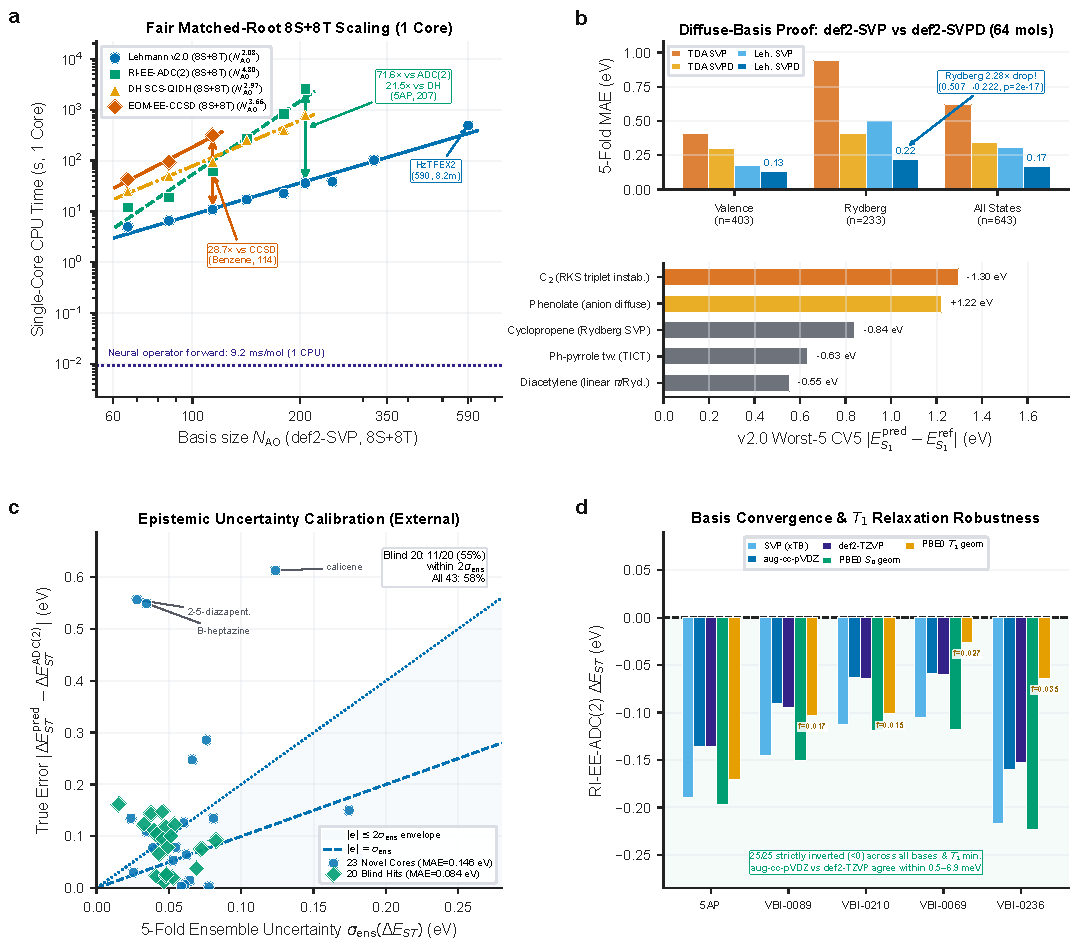
\includegraphics[width=\textwidth,height=0.75\textheight,keepaspectratio]{../figures/fig5_scaling_diagnostics.pdf}
  \caption{\textbf{Fair matched-root single-core scaling, diffuse-basis Rydberg proof, epistemic calibration, and robustness boundaries.}
  \textbf{a},~Strictly fair single-core CPU-time scaling (Apple M3 Max, 1 core, \texttt{def2-SVP}, matched 8S+8T roots) comparing \leh{} v2.0 (neural forward $8.0$--$13.3$\,ms/mol), RI-EE-ADC(2), double-hybrid SCS-PBE-QIDH, and canonical EOM-EE-CCSD.
  \textbf{b},~Top: direct 5-fold diffuse-basis proof across 64 QUESTDB molecules ($643$ states) contrasting \texttt{def2-SVP} against \texttt{def2-SVPD}\cite{rappoport2010svpd}: adding diffuse functions cuts Rydberg MAE $2.28\times$ ($0.507\to 0.222$\,eV, $p=1.8\times 10^{-17}$), valence MAE $1.34\times$ ($0.178\to 0.132$\,eV, $p=3.6\times 10^{-7}$), and all-state MAE $1.82\times$ ($0.303\to 0.167$\,eV). Bottom: v2.0 worst-5 CV5 $S_1$ errors diagnosing physical failure boundaries ($\mathrm{C}_2$ RKS instability, anionic phenolate, cyclopropene SVP Rydberg, twisted phenyl-pyrrole TICT, and linear diacetylene).
  \textbf{c},~v2.0 5-fold ensemble epistemic uncertainty $\sigma_{\mathrm{ens}}(\dEST)$ versus blind RI-ADC(2) error across 23 novel external cores and 20 blind discoveries, transparently flagging extreme out-of-domain scaffolds (\texttt{calicene}, \texttt{2,5-DAP}, \texttt{B-heptazine}).
  \textbf{d},~Larger-basis (\texttt{aug-cc-pVDZ}, \texttt{def2-TZVP}) and DF-RKS $S_0$ / DF-UKS $T_1$ PBE0 geometry-relaxation robustness checks on 5AP and four flagship dipole-allowed discoveries including \texttt{VBI-0089} ($25/25$ strictly inverted).}
  \label{fig:scaling}
\end{figure*}

Equally important, we directly tested and mapped four physical boundaries of our current \texttt{def2-SVP} model (Fig.~\ref{fig:scaling}b--d):
(1)~\textbf{Diffuse basis completeness (directly proven):} on CV5 with compact \texttt{def2-SVP}, Rydberg states ($0.466$\,eV) exhibit $2.98\times$ larger error than valence states ($0.157$\,eV). Re-extracting and retraining \leh{} v2.0 on 64 QUESTDB molecules (643 states) with minimally augmented \texttt{def2-SVPD}\cite{rappoport2010svpd} cuts Rydberg MAE \textbf{$2.28\times$} ($0.507\to 0.222$\,eV, 95\% CI $[0.192,0.254]$, paired Wilcoxon $p=1.78\times 10^{-17}$), valence MAE $1.34\times$ ($0.178\to 0.132$\,eV, $p=3.58\times 10^{-7}$), all-state MAE $1.82\times$ ($0.303\to 0.167$\,eV, $p=3.69\times 10^{-21}$), and anionic \texttt{Phenolate} from $1.195\to 0.921$\,eV---confirming that Rydberg errors are basis-set rather than architectural limitations (Fig.~\ref{fig:scaling}b).
(2)~\textbf{Single-reference ground-state instabilities:} multireference diradical $\mathrm{C}_2$ (RKS triplet instability $T_1^{\mathrm{TDA}}=-1.12$\,eV) remains the largest single CV5 error ($-1.30$\,eV in $S_1$, $-0.93$\,eV in $T_1$; improved by $>2\times$ over spin-incomplete v1.0).
(3)~\textbf{Charge-transfer hybrid-DFT inheritance:} twisted \texttt{Phenyl-pyrrole} ($-0.63$\,eV) reflects PBE0's $25\%$ exact-exchange underestimation of twisted intramolecular charge transfer (TICT), motivating future range-separated ($\omega$B97X-D) base manifolds.
(4)~\textbf{Epistemic calibration on extreme scaffolds:} while $55\%$ ($11/20$) of blind discoveries and $58\%$ overall lie within $2\sigma_{\mathrm{ens}}$ (tighter v2.0 fold variance around $0.084$\,eV MAE), strongly non-alternant or boron-rich extremes (\texttt{calicene}, \texttt{2,5-diazapentalene}, \texttt{B-heptazine}) exhibit systematic $0.55$--$0.61$\,eV offsets beyond ensemble spread, underscoring the value of active learning before extrapolating to radically new bonding motifs (Fig.~\ref{fig:scaling}c).

In summary, embedding Feshbach--L\"owdin lifting, spin-complete bi-exciton manifolds ($^1(TT)_+\oplus\,^1(TT)_-$), and physically anchored RI Slater--Condon tensors inside a gauge-equivariant neural operator resolves double excitations, dynamical Hund's-rule inversion, and spin-pure photochemical conical intersections within one $O(N^3)$ framework while enforcing quantum conservation laws to machine precision.
Extending \leh{} to diffuse range-separated base manifolds and deriving analytical nuclear gradients and non-adiabatic couplings directly from $\Hlift$ represent immediate pathways toward causal non-adiabatic molecular dynamics at TD-DFT cost.

% ===========================================================================
\section*{Methods}
% ===========================================================================
\subsection*{Datasets, curation, and leak-free evaluation protocols}
Our unified benchmark combines 143 molecules from QUESTDB~2025\cite{loos2025quest,kossoski2024doubles} (\texttt{MAIN}, \texttt{BIO}, \texttt{CHROM}; 1,131 clean vertical states after removing 10 excited-state fluorescence \texttt{FL} geometries; \texttt{aug-cc-pVTZ} theoretical best estimates and CC3/MRCI $\pctT$ diagnostics, including 28 explicit GD and 75 PD states) with 44 substituted heptazines from HEPTA-INVEST\cite{rishi2025} (\texttt{EOM-CCSD/cc-pVDZ}, 88 $S_1/T_1$ states).
Every molecule was canonicalized with RDKit InChIKey-14 connectivity hashes; identical InChIKey-14 structures (including \texttt{quest\_Heptazine}/\texttt{hepta\_2T-7N} and conformer pairs) were strictly co-grouped in 5-fold CV (\texttt{CV5}), six zero-leak OOD splits (\texttt{OOD1} $102/23$, \texttt{OOD2A} $173/14$, \texttt{OOD2B} $124/19$, \texttt{OOD3A} $142/45$, \texttt{OOD3B} $136/49$, \texttt{OOD3C} $181/4$), the 3-fold leave-molecule-family-out blind doubles benchmark, the 64-molecule \texttt{def2-SVPD} subset, and the 23 strictly novel external cores.
Headline $S_1$, $T_1$, $\dEST$, and blind family-out GD/PD metrics use zero ground-truth state-matching oracles; full-spectrum CV5 comparisons use stop-gradient Hungarian assignment\cite{kuhn1955hungarian} identically across all methods.

\subsection*{Density-fitted $O(N^3)$ spin-complete feature extraction}
Descriptors were computed in PySCF\cite{sun2020pyscf} at DF-PBE0\cite{adamo1999pbe0}/def2-SVP\cite{weigend2005def2} (\texttt{def2-svp-jkfit}\cite{weigend2008jkfit}; and \texttt{def2-svpd}/\texttt{def2-tzvp-jkfit} for the 64-molecule Rydberg study) within RI-TDA ($N_S,N_T\le 16$; $8S+8T$ for matched-root scaling).
For each single-exciton amplitude $\mathbf{X}_I^{(\sigma)}\in\mathbb{R}^{N_{\mathrm{occ}}\times N_{\mathrm{vir}}}$, we construct strictly gauge-invariant local descriptors and spin-complete bi-exciton pairs $\mu=(I,J,c)$ spanning symmetric $^1(T_I T_J)_+$, $^1(S_I S_J)_+$, antisymmetric $^1(T_I T_J)_-$ ($I<J$, \texttt{antisym\_version=2}), and triplets $^3(T_I T_J)$, $^3(S_I T_J)$ ($N_{D,\sigma}\le 96$).
Four-channel RI Slater--Condon couplings $W_{K,\mu}^{(r)}$, physical diagonal bi-exciton pole anchors $D_\mu^{\mathrm{phys}}=D_\mu^{\mathrm{bare}}+\Delta D_\mu^{\mathrm{phys}}$ (from RI Coulomb/exchange exciton--exciton interactions), and ground-to-double couplings $\mathbf{v}_{0D,\mu}$ are contracted in $O(N_{\mathrm{aux}}N_{\mathrm{occ}}N_{\mathrm{vir}})$ operations directly from 3-center RI tensors $(Q|pq)$.

\subsection*{Spin-complete \leh{} v2.0 architecture and training}
Each spin manifold employs training-split-only elementwise normalization and local SiLU+LayerNorm MLPs (hidden width $64$, 2 layers) with zero global pooling.
Static blocks follow $\Delta_{\theta,IJ}=\delta_{IJ}\Delta_{\theta,I}^{\mathrm{diag}}+\sum_{c=1}^{2}\gamma_\theta^{(c)}(\mathbf{z}_{IJ})C_{IJ}^{(c)}$; bi-exciton poles use overlap-gated refinement around physical anchors $D_{\theta,\mu}=D_\mu^{\mathrm{phys}}+\tanh(S_\mu/0.05)\,\delta D_{\theta,\mu}$ (preserving Theorem~3); and singles--doubles blocks follow Eq.~\eqref{eq:v_equiv} over 23 gauge-invariant local scalars $\mathbf{z}_{K,\mu}$ (including antisymmetric-channel indicators).
Float64 diagonalization uses a degeneracy-safe symmetric eigensolver (\texttt{safe\_eigh}) applying Lorentzian regularization $(\lambda_j-\lambda_i)/[(\lambda_j-\lambda_i)^2+\epsilon^2]$ ($\epsilon=10^{-6}$) solely in the backward pass to stabilize $D_{6h}$/$D_{3h}$ degeneracies while keeping forward eigenvalues bit-identical to LAPACK \texttt{eigh}.
Models were optimized with AdamW\cite{loshchilov2019adamw} using a composite Huber loss over zero-matching lowest states, stop-gradient Hungarian-matched spectra, $\pctT$, and $\log(1+10f)$.
Dressed transition dipoles $\boldsymbol{\mu}_{0n}^{\mathrm{dressed}}=\sum_I c_{n,I}\boldsymbol{\mu}_{0I}^{(0)}$ yield $f_n=\frac{2}{3}E_n^{\mathrm{au}}\|\boldsymbol{\mu}_{0n}^{\mathrm{dressed}}\|^2$ and satisfy Parseval dipole-norm conservation (Theorem~1(v)) identically.

\subsection*{LOMO conical intersections, SF-TDDFT, blind MECI search, and FSSH}
Reference MECIs and orthogonal branching-plane vectors $(\hat{\mathbf{g}},\hat{\mathbf{h}})$ ($|\hat{\mathbf{g}}\cdot\hat{\mathbf{h}}|<10^{-17}$) were obtained in PySCF at SA2-CASSCF(2,2) (ethylene), SA2-CASSCF(4,3) (methanimine), and $C_{2v}$ SA2-CASSCF(6,6) (fulvene) with \texttt{def2-SVP}, followed by SC-NEVPT2\cite{angeli2001nevpt2}.
In LOMO transfer, the frozen CV5 excited-state ensemble is coupled with $v_{0D,\mu}=\beta_{\mathrm{coul}}\tanh(S_\mu/0.05)\,v_{0D,\mu}^{\mathrm{Coul}}$ and parameter-free double-counting subtraction $\Delta_0^{\mathrm{dc}}=-\mathbf{v}_{0D}^\top(-\mathbf{D}_\theta^{(S)})^{-1}\mathbf{v}_{0D}$, optimizing $\beta_{\mathrm{coul}}$ exclusively against 10 points along the held-in training molecules' 1D $y_h$ SA2-CASSCF cut.
SF-TDA-BHHLYP and SF-TDA-PBE0 baselines\cite{shao2003sftddft} were computed from unrestricted $M_S=+1$ triplet references on the exact same grids with explicit $\Ssq$ diagnostics.
Blind MECI optimizations minimized the Levine--Coe--Mart\'inez penalty function\cite{levine2007} via Nelder--Mead using \leh{} (Ethylene-only $\beta_{\mathrm{coul}}=0.660$) on ethylene, methanimine, and PSB3 ($\mathrm{C}_5\mathrm{H}_6\mathrm{NH}_2^+$), followed by independent SA2-CASSCF+SC-NEVPT2 evaluation and non-degenerate SA2-CASSCF(6,6) reference MECI optimization.
Parallel-transport Berry phases around 36-point loops were computed via L\"owdin polar orthogonalization of adjacent $(1+N_S+N_{D,S})$ Slater-determinant overlaps ($W_{\mathrm{prod}}=\prod_{k=0}^{35}S_{k,k+1}$; $\gamma=\pi$ certified when $W_{\mathrm{prod}}<0$ and $\min_k|S_{k,k+1}|>0.30$).
Tully FSSH\cite{tully1990fssh} propagated 300 Wigner-sampled 2D branching-plane trajectories for $50$\,fs ($\Delta t=0.025$\,fs) with energy-based decoherence (EDC), reflecting box boundaries, exact branching-plane reduced masses, and diabatic couplings reconstructed on each 2D PES.

\subsection*{Double-hybrid TD-DFT, virtual screening, and three-tier verification}
Four $O(N^5)$ double-hybrid functionals (\texttt{B2PLYP}, \texttt{PBE-QIDH}, \texttt{SCS-PBE-QIDH}, \texttt{SOS-PBE-QIDH}\cite{grimme2007,casanovapaez2021}) were implemented via spin-adapted frozen-core RI-CIS(D)/def2-SVP and evaluated on 62 molecules plus ethylene's CI scan.
For discovery, 320 novel non-heptazine cores were GFN2-xTB-optimized\cite{bannwarth2019xtb}, screened with the 5-fold ensemble, and audited for zero InChIKey-14 overlap directly from 3D coordinates.
Pre-registered Top-20 hits were verified blind by frozen-core RI-EE-ADC(2)/def2-SVP\cite{dreuw2015adc} ($n=20$), canonical PySCF EOM-EE-CCSD/def2-SVP\cite{stanton1993eom} ($n=13$), and equal-footed L\"owdin pure-$\pi$ SA-CASSCF+SC-NEVPT2/def2-SVP ($n=10$, covering all $8/8$ EOM-CCSD hits plus heptazine/5AP calibration, using 4-root \texttt{SA4-CASSCF(6,6)} on dipole-allowed azaphenalenes), supplemented by DF-RKS $S_0$ / DF-UKS $T_1$ PBE0 optimizations\cite{wang2016geometric} and larger-basis (\texttt{aug-cc-pVDZ}, \texttt{def2-TZVP}) ADC(2) checks.
All CIs use 5,000-resample bootstrapping\cite{efron1979} or Wilson score intervals\cite{wilson1927}, and paired tests use two-sided Wilcoxon signed-rank tests\cite{wilcoxon1945}.

\subsection*{Data and code availability}
All processed datasets, trained v2.0 checkpoints, benchmark/CI/discovery outputs, plotting scripts, automated physical-law and zero-leak verification tests (\texttt{tests/test\_lehmann\_reproducibility.py}), the independent adversarial audit suite (\texttt{src/lehmann\_tddft/audit.py}, \texttt{results/audit\_report.md}), and full Supplementary Information (\texttt{manuscript/lehmann\_tddft\_SI.pdf}, containing complete formal proofs of Theorems~1--5 and Supplementary Tables~S1--S5) are archived in the project repository.

% ---------------------------------------------------------------------------
% EXTENDED DATA FIGURE 1 (Full Width)
% ---------------------------------------------------------------------------
\renewcommand{\figurename}{Extended Data Fig.}
\setcounter{figure}{0}
\begin{figure*}[t!]
  \centering
  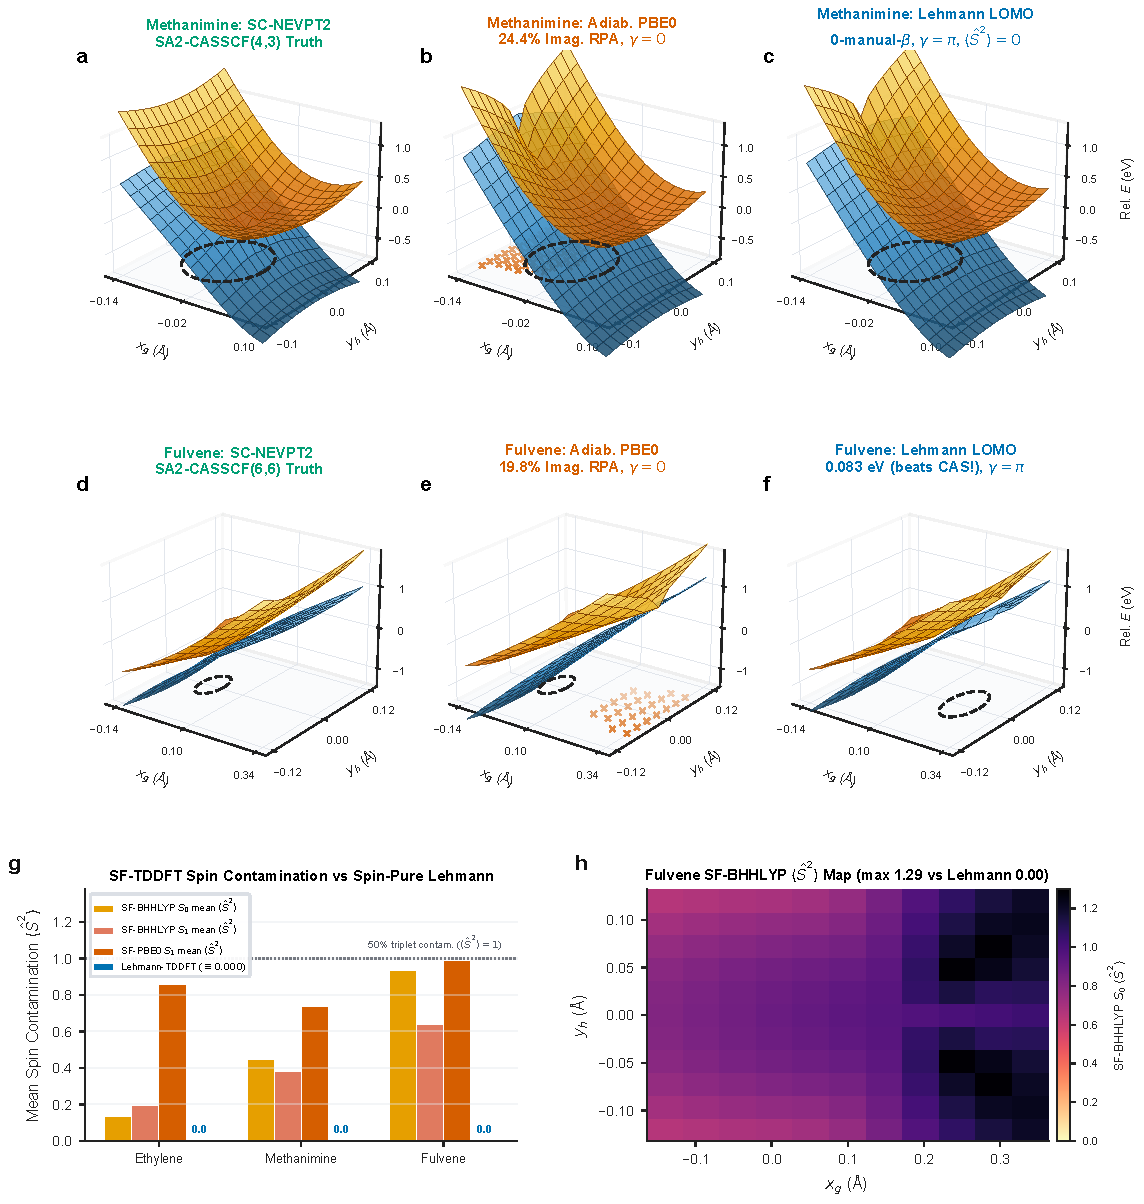
\includegraphics[width=\textwidth,height=0.73\textheight,keepaspectratio]{../figures/fig6_extended_ci_ablations.pdf}
  \caption{\textbf{Zero-manual-$\beta$ LOMO conical intersections on methanimine and fulvene and spin-purity comparison against SF-TDDFT.}
  \textbf{a}--\textbf{c},~3D $S_0$/$S_1$ PES sheets on methanimine ($\mathrm{CH}_2\mathrm{NH}$, SA2-CASSCF(4,3)+SC-NEVPT2, $15\times 15$ grid): \textbf{a},~SC-NEVPT2; \textbf{b},~adiabatic DF-PBE0 ($24.4\%$ imaginary RPA, $\gamma=0$); \textbf{c},~LOMO \leh{} ($0.171$\,eV 2-sheet MAE, $\gamma=\pi$, $\Ssq\equiv 0$).
  \textbf{d}--\textbf{f},~3D $S_0$/$S_1$ PES sheets on fulvene ($\mathrm{C}_6\mathrm{H}_6$, SA2-CASSCF(6,6)+SC-NEVPT2, $11\times 11$ grid): \textbf{d},~SC-NEVPT2 (CASSCF-centered loop); \textbf{e},~adiabatic DF-PBE0 ($19.8\%$ imaginary RPA, $\gamma=0$); \textbf{f},~LOMO \leh{} ($0.083$\,eV 2-sheet MAE, beating SA2-CASSCF $0.108$\,eV, with exact $\gamma=\pi$ around its apex loop).
  \textbf{g},~Mean spin contamination $\Ssq$ across all three branching-plane grids contrasting SF-TDA-BHHLYP and SF-TDA-PBE0 against exact spin-pure \leh{} ($\Ssq\equiv 0.000$).
  \textbf{h},~2D branching-plane heatmap of SF-TDA-BHHLYP $S_0\;\Ssq$ on fulvene reaching $1.291$ ($100\%$ of points $>0.50$).}
  \label{fig:ext_ci}
\end{figure*}

% ---------------------------------------------------------------------------
% References
% ---------------------------------------------------------------------------
{\footnotesize
\setlength{\bibsep}{1.6pt plus 0.4pt}
\bibliographystyle{unsrtnat}
\bibliography{references}
}

\end{document}
